    \documentclass[conference]{IEEEtran}

    \usepackage{amsmath,amssymb,amsfonts}
    \usepackage{graphicx}
    \usepackage{cite}
    \usepackage{algorithm}
    \usepackage{algorithmic}
    \usepackage{array}
    \usepackage{booktabs}

    \title{Fault-Tolerant and Load-Balanced IIoT Edge--Fog Architecture}

    \author{
    \IEEEauthorblockN{
    Benyapa Tawunwoot\IEEEauthorrefmark{1},
    Proud Pitugkittikul\IEEEauthorrefmark{2},
    Ramona Bhuthontharaj\IEEEauthorrefmark{3},\\
    Nang Yein Mo Hsai\IEEEauthorrefmark{4},
    Somchart Fugkeaw\IEEEauthorrefmark{5}
    }
    \IEEEauthorblockA{
    School of Information, Computer, and Communication Technology (ICT)\\
    Sirindhorn International Institute of Technology (SIIT), Thammasat University, Thailand\\
    Email:
    \IEEEauthorrefmark{1}6622770509@g.siit.tu.ac.th,
    \IEEEauthorrefmark{2}6622770665@g.siit.tu.ac.th,
    \IEEEauthorrefmark{3}6622782140@g.siit.tu.ac.th,\\
    \IEEEauthorrefmark{4}m6822041015@g.siit.tu.ac.th,
    \IEEEauthorrefmark{5}somchart@siit.tu.ac.th
    }
    }


    \begin{document}

    \maketitle

    \begin{abstract}
    This paper proposes a fault-tolerant and load-balanced Industrial Internet of Things (IIoT) edge--fog architecture for secure, storage-efficient data processing with fault-resilient operation. The framework combines fog-scoped AES key isolation enforced by Trusted Execution Environments (TEEs), Paillier homomorphic slot aggregation, gossip-based adaptive load balancing, and sensor-side ACK-based fault detection. Fog nodes exchange status through a decentralized gossip protocol and check the most recent workload table on every incoming sensor reading. Overload is handled through KMM-provisioned enclave delegation without sensor retransmission, while ACK timeout allows sensors to redirect encrypted readings after fog silence and notify the KMM for delegated key provisioning. Vacated aggregation slots are filled with Paillier encryptions of zero, preserving aggregate correctness under mid-window delegation. The proposed scheme jointly supports fog-scoped key isolation, adaptive per-reading delegation, bounded-loss ACK-based recovery, and storage-efficient aggregation: one ciphertext per window regardless of sensor count. The 500~ms aggregation window is satisfied in non-delegation windows; delegation windows incur an additional 150~ms for TEE key provisioning.
    \end{abstract}

    \begin{IEEEkeywords}
    Industrial Internet of Things, Edge--fog computing, Fault tolerance, Load balancing, Trusted execution environment, Paillier encryption, Key management
    \end{IEEEkeywords}

    \section{Introduction}
    The Industrial Internet of Things (IIoT) has become a foundational 
    pillar of Industry~4.0, enabling continuous monitoring, predictive 
    maintenance, and automated control across large-scale industrial 
    environments~\cite{tange2020}. Numerous sensors and control devices 
    generate time-sensitive data streams that impose strict requirements 
    on latency, reliability, and security. For example, vibration sensors 
    on rotating machinery produce hundreds of measurements per second, 
    while safety monitoring systems in chemical plants must detect 
    abnormal conditions in real time to prevent hazardous 
    incidents~\cite{farooq2023}.

    Centralized cloud architectures struggle to satisfy these latency 
    requirements due to the long communication path between sensors and 
    remote data centers. Edge and fog computing have emerged as the 
    dominant solution, moving computation closer to data 
    sources~\cite{jin2024}. In an edge--fog architecture, fog nodes
    perform preprocessing near IIoT devices and provide intermediate
    aggregation and analytics before forwarding results to the cloud,
    significantly reducing latency and bandwidth overhead.

    Despite these advantages, fog-based IIoT deployments face three 
    critical challenges. First, heterogeneous fog nodes subject to static 
    workload assignment create resource imbalance, where weaker nodes 
    become overloaded while stronger nodes remain 
    underutilized~\cite{kashani2023}. Second, fault-tolerance mechanisms in fog environments introduce extra computational and storage overhead, which affects performance in resource-constrained settings~\cite{chen2024lb}. Third, many 
    existing systems require fog nodes to decrypt sensor data before 
    performing aggregation, violating the zero-trust assumption of modern 
    distributed infrastructures and exposing sensitive industrial data at 
    the fog layer~\cite{mirani2022}.

    Prior work addresses each challenge independently but creates new 
    tradeoffs when combined. Global shared AES key schemes allow 
    efficient key management but mean that a single compromised fog node 
    exposes all sensor data across the entire deployment. Per-reading 
    Paillier encryption~\cite{peng2022} preserves fog-layer privacy but 
    transmits $n$ ciphertexts per window to the cloud, causing storage 
    overhead that grows linearly with sensor count. Replication-based 
    fault tolerance ensures service continuity but duplicates 
    already-large ciphertexts, amplifying the storage problem. No 
    existing work eliminates all three tradeoffs within a single unified 
    architecture.

    To address these limitations, this paper proposes a fault-tolerant
    and load-balanced IIoT edge--fog architecture. The proposed framework
    integrates fog-scoped AES key isolation enforced by Trusted Execution
    Environments (TEEs)~\cite{costan2016}, Paillier homomorphic slot
    aggregation~\cite{paillier1999}, and gossip-based adaptive load
    balancing, providing end-to-end data confidentiality without exposing
    plaintext at any intermediate processing stage.

    The primary novelty of this work is the integration of fog-scoped key
    isolation with a three-layer fault-handling hierarchy for fog-based
    IIoT. Each fog node holds only its own scoped AES key $k_{fogI}$ sealed
    inside the TEE hardware, while temporary delegation is performed by the KMM
    provisioning the delegating node's scoped key to the receiving enclave
    for one aggregation window and revoking it after the window closes. The
    hierarchy combines: (i) fog-initiated TEE delegation when self-detected
    workload exceeds threshold $\tau$, providing immediate and zero-data-loss
    overload handling; (ii) sensor-initiated ACK-timeout redirect using the
    local gossip table and a task-aware capacity scoring selector (CapacityScore,
    defined in Section~\ref{sec:lb}) with KMM provisioning in approximately
    $150\,ms$; and (iii) gossip-based neighbor detection as a fallback for
    simultaneous fog-node and sensor--fog channel failure.

       \section{Related Work}

This section reviews existing literature across three areas: (A) load balancing in fog environments, (B) fault tolerance mechanisms for distributed fog systems, and (C) privacy-preserving data processing in IIoT and fog computing.

\subsection{Load Balancing in Fog Computing}

Load balancing in fog computing is concerned with distributing incoming workloads efficiently across available nodes to prevent bottlenecks and maximise resource utilisation~\cite{kashani2023}. The challenge is compounded by the heterogeneous capacity of fog nodes which differ in CPU, memory, and network bandwidth and by the diversity of IIoT task types, which impose widely varying computational demands. Recent surveys identify three dominant strategy families: centralised scheduling, decentralised peer-to-peer coordination, and gossip-based dissemination~\cite{vijarania2025,nemati2024}.

\subsubsection{Optimisation-Based Approaches}

Early optimisation-based methods applied metaheuristics such as Particle Swarm Optimisation and Ant Colony Optimisation to allocate workflows across fog nodes~\cite{tripathy2026}. The FOCALB architecture combined fitness-based node selection with fog-aware scheduling to reduce execution time and energy consumption for scientific workflow applications~\cite{kaur2021}. While FOCALB demonstrated the value of capacity-aware routing, it targets batch workflows rather than the continuous, high-frequency sensor streams characteristic of IIoT deployments, and provides no mechanism for differentiating among task types with heterogeneous computational profiles.

Multi-criteria decision-making frameworks extended optimisation approaches by jointly evaluating CPU load, network latency, and queue depth. Ebrahim and Hafid proposed an ELECTRE-based outranking method that ranks fog nodes by pairwise concordance and discordance across multiple criteria~\cite{ebrahim2023b}. Although this approach produces theoretically principled decisions, its $\mathcal{O}(N^2)$ pairwise comparison complexity is prohibitive under high IIoT task arrival rates. The authors explicitly deployed the method on resource-rich SDN controllers, introducing a centralised coordinator that becomes a single point of failure. A follow-up hybrid model combining FAHP and FTOPSIS improved utilisation in fog-cloud simulations~\cite{ahmed2024} but similarly assumed a centralised control plane. Walia et al.\ proposed an adaptive multi-criteria framework for fog-cloud resource allocation that achieved load balance improvements over conventional round-robin and threshold baselines~\cite{walia2024}; however, their weight assignment relied on expert judgement rather than empirical calibration against measured sensor workloads, limiting applicability to heterogeneous IIoT environments.

\subsubsection{Reinforcement Learning Approaches}

Reinforcement learning has been applied to fog load balancing to handle dynamic workloads without static scheduling rules. Ebrahim and Hafid proposed a Double Deep Q-Learning agent that minimises waiting time while preserving node-load privacy in multi-provider deployments~\cite{ebrahim2023a}. More recently, the same group extended this to a fully distributed Multi-Agent Reinforcement Learning (MARL) framework in which agents operate within local collaboration regions, incorporating a gossip-based observation protocol to address the impracticality of real-time global state visibility~\cite{ebrahim2025}. While MARL improves scalability compared to centralised RL, these approaches require an offline training phase and may need retraining when network topology or task arrival distributions change---a significant limitation in safety-critical IIoT systems where operational continuity is mandatory. Furthermore, neither the RL nor the MARL formulations differentiate among sensor types: vibration, pressure, temperature, and flow sensors are treated as a homogeneous task class despite their substantially different computational demands.

\subsubsection{Gossip-Based and Decentralised Approaches}

Gossip protocols have attracted attention for fog load management because they disseminate status information among nodes through random pairwise exchanges without requiring a central coordinator. Kashani et al.\ surveyed gossip and epidemic-style load balancing mechanisms, noting their low per-node message overhead and natural scalability but identifying their limited integration with task-aware delegation policies as an open problem~\cite{kashani2020}. A recent systematic literature review covering 113 peer-reviewed studies from 2020 to 2024 confirmed that gossip-based coordination remains predominantly used for monitoring rather than as a complete scheduling substrate, and highlighted the lack of heterogeneous task-type differentiation as a critical gap across the field~\cite{vijarania2025}.

A key limitation shared by all three strategy families is their treatment of tasks as homogeneous units, typically classified only by delay sensitivity. In practice, IIoT workloads differ substantially: a vibration sensor task involving FFT-based spectral analysis is compute-intensive ($\mathcal{O}(n \log n)$), whereas a temperature monitoring task involves only threshold evaluation ($\mathcal{O}(n)$). Assigning identical routing weights to these tasks leads to suboptimal delegation decisions, particularly under heterogeneous node configurations. The proposed framework addresses this gap by introducing a CapacityScore formula with two delay-class weight configurations and a task-type compatibility term---a BW-prioritized, latency-sensitive configuration for time-critical tasks and a $\phi^2$-penalised CPU-compatibility configuration for compute-heavy tasks---adapting delegation decisions to the computational and structural profile of each task class without requiring a centralised controller.

\subsection{Fault Tolerance in Fog Computing}

Fog environments are susceptible to node failures caused by hardware faults, network instability, or transient resource exhaustion. A comprehensive 2024 taxonomy of fault-tolerance approaches in distributed and cloud computing organised existing methods into reactive, proactive, adaptive, and hybrid categories~\cite{kirti2024}. In the fog context, the dominant techniques remain replication, checkpointing, and resubmission-based scheduling.

\subsubsection{Replication and Checkpointing}

Replication-based methods maintain backup copies of tasks across multiple fog nodes so that computation can continue when a primary node fails. Liu et al.\ proposed a replica-based scheduling strategy for heterogeneous cloud-fog environments that minimises the number of replicas needed while satisfying reliability constraints~\cite{liu2024}. Rajab and Younis introduced a dynamic fault-tolerant scheduling scheme combining checkpointing and replication that periodically stores task states, enabling recovery without full restart when failures occur~\cite{rajab2021}. Both approaches have demonstrated reliability improvements; however, they introduce additional storage overhead and computational cost proportional to the replication factor, which is problematic for resource-constrained fog nodes. Furthermore, these methods address load balancing and fault tolerance as separate concerns, leading to fragmented system designs and increased coordination overhead.

\subsubsection{Metaheuristic and ML-Based Fault-Tolerant Scheduling}

Hybrid metaheuristic methods have been proposed to jointly optimise workload distribution and fault-tolerant scheduling. Ghasemi proposed the MOHHO algorithm combining Modified Harris Hawks Optimisation with multi-objective service placement in fog computing, which identifies critical tasks and selectively applies replication or resubmission strategies upon node failure~\cite{ghasemi2024}. While these approaches improve reliability, they require offline parameter tuning and incur convergence overhead that may delay task reassignment under real-time failure conditions. Merah et al.\ applied a deep-learning and genetic-algorithm clustering approach to load balancing in IoT edge environments, showing adaptive traffic distribution under workload fluctuations~\cite{merah2025}; however, their framework targets traffic load distribution rather than fault-tolerant task recovery, and does not address mid-window state preservation under node failure. Mohammadi et al.\ studied fault tolerance specifically in fog-based Social IoT environments and highlighted that combining failure detection with load redistribution in a unified lightweight mechanism remains an open challenge~\cite{mohammadi2023}.

\subsubsection{Gossip-Based Failure Detection}

Gossip protocols were originally proposed for distributed database maintenance and epidemic information dissemination~\cite{demers1988epidemic}. Their application to failure detection in fog networks follows naturally from their decentralised nature: nodes declare a peer unavailable when it fails to respond for a predefined number of consecutive gossip rounds, without requiring a centralised health monitor. Naha et al.\ proposed a fuzzy logic-based failure handling mechanism built on gossip-style status exchange for fog nodes~\cite{naha2021}, demonstrating that decentralised detection can adapt robustly to varying failure rates. However, this work did not integrate failure detection with task-aware load balancing in a unified scheduling framework.

The proposed framework addresses the gap between fault detection and scheduling by combining gossip-based failure detection with the same CapacityScore delegation mechanism used for overload-driven load balancing. When a node is declared unavailable after missing $r$ consecutive gossip rounds, its pending tasks are reassigned to the highest-scoring available neighbour using the most recently maintained gossip state table, requiring no additional inter-node communication beyond what is already exchanged for load monitoring.

\subsection{Privacy-Preserving Data Processing in IIoT and Fog Computing}

Protecting sensitive IIoT sensor data during transit and processing at intermediate fog nodes is a central security requirement. Prior work has explored symmetric encryption at the sensor layer, privacy-preserving aggregation at fog nodes, and hybrid cryptographic pipelines combining these primitives.

\subsubsection{Homomorphic Encryption for Fog Aggregation}

Homomorphic encryption enables computation directly on ciphertexts without decryption, making it suitable for privacy-preserving aggregation at fog nodes. Zhang et al.\ proposed a Paillier-based privacy-preserving aggregation scheme in fog computing that demonstrated fault tolerance by handling false data injection through blinding factor adjustments~\cite{zhang2018}. Shang et al.\ combined Paillier homomorphic encryption with ECDSA signatures to build a fault-tolerant data aggregation scheme that resists collusion attacks between the fog node and the cloud~\cite{shang2023}. A recent fog-enabled secure analytics framework (FESDAO) extended Boneh-Goh-Nissim homomorphic encryption to support not only summation but statistical operations mean, variance, and ANOVA directly on encrypted data at the fog layer, without requiring decryption before analysis~\cite{fesdao2025}. These works collectively confirm the feasibility of fog-layer homomorphic aggregation; however, none addresses the dynamic workload delegation scenario in which sensors are reassigned mid-aggregation-window, which is central to the proposed framework.

The MOZAIK platform demonstrated an end-to-end privacy-preserving IoT-to-cloud architecture using both Secure Multi-Party Computation and Fully Homomorphic Encryption, showing that encrypted data pipelines can satisfy practical latency requirements~\cite{januszewicz2025}. However, MOZAIK targets cloud-centralised analytics and does not incorporate fog-layer load balancing or mid-window delegation semantics. The proposed framework directly addresses this gap by introducing a slot protocol that maintains aggregate correctness under dynamic sensor reassignment, using zero-fill ciphertexts to preserve IND-CPA indistinguishability of vacated slots.

\subsubsection{Hybrid Cryptographic Pipelines}

Practical IIoT systems increasingly combine symmetric, asymmetric, and homomorphic primitives into layered pipelines that balance security with performance. Qin et al.\ surveyed proxy re-encryption schemes and showed that PRE-based delegation achieves sub-15~ms overhead for typical IIoT payloads on commodity fog hardware~\cite{qin2022}, validating delegation latency as a practical concern. However, PRE requires key material to be present at an intermediate node during re-encryption, which creates a trust boundary conflict in hostile-fog threat models.

The proposed framework replaces the PRE delegation layer with a Trusted Execution Environment (TEE) channel implemented via Intel SGX enclaves and a Key Management Module. This eliminates the need for the intermediate node to hold re-encryption key material in host memory, bounding the blast radius of fog node compromise to a single fog-scoped key group. This design follows the direction identified by recent surveys on secure fog computing, which emphasise hardware-rooted trust as the emerging approach for overcoming the limitations of software-only delegation schemes~\cite{nemati2024,kumar2023}.

    \section{Preliminaries}
    \subsection{System Architecture}
    \label{sec:arch}
    \begin{figure}[htbp]
    \centering
    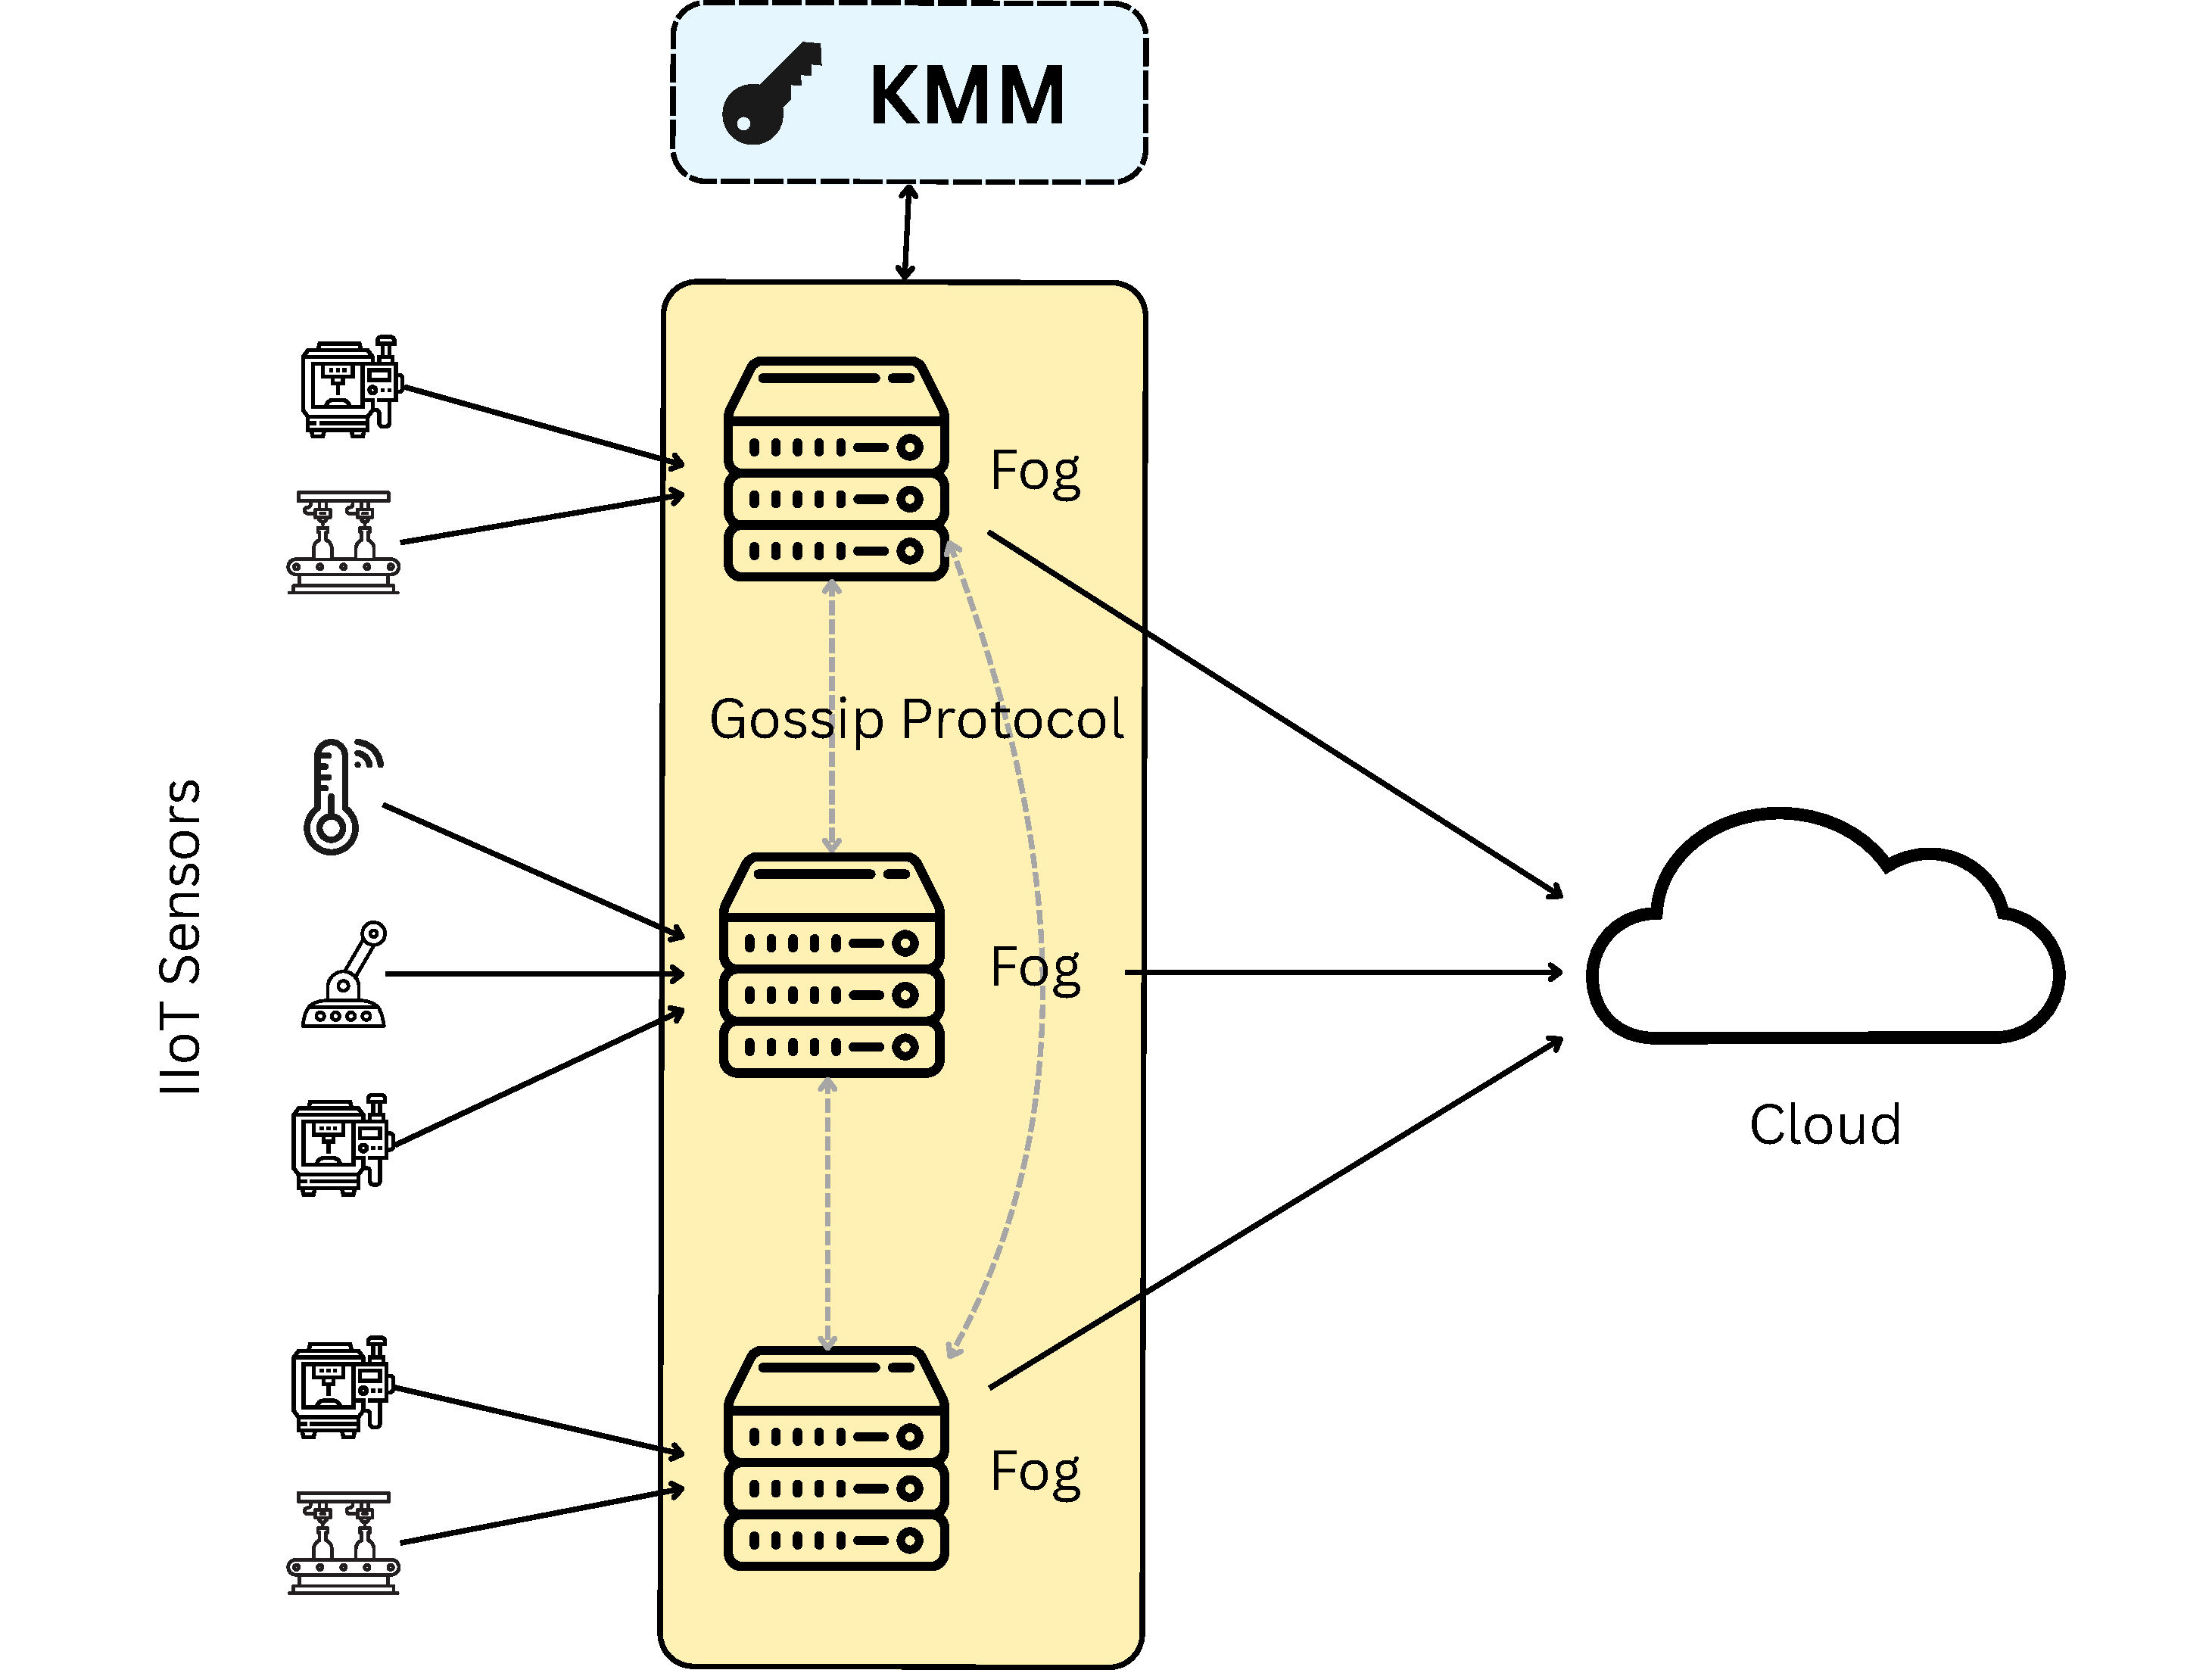
\includegraphics[width=1.0\linewidth]{../figures/overall_diagram.pdf}
    \caption{Architecture of the proposed secure IIoT fog–cloud framework.}
    \label{fig:architecture}
    \end{figure}
    As shown in Fig.~\ref{fig:architecture}, the proposed system consists of five layers: the IIoT sensor layer, fog TEE enclave layer, fog Paillier aggregation layer, fog load-balancing layer, and cloud storage layer. The key management module (KMM) additionally performs a lightweight window-combine step that receives one Paillier aggregate from each fog node every $W=500\,ms$ and combines them homomorphically.

    \begin{itemize}
        \item \textbf{IIoT Sensor Layer}: IIoT sensors collect environmental or industrial monitoring data. Each sensor sends four AES-128-GCM encrypted readings per aggregation window (one every 125~ms) using the fog-scoped key of its assigned fog node. With 100~sensors across five fog nodes (20~per node), this yields 400~readings per 500~ms window.
        \item \textbf{Fog TEE Enclave Layer}: Each fog node first verifies the AES-GCM authentication tag of incoming sensor readings using its provisioned fog-scoped key, rejecting readings whose tag fails verification. Accepted ciphertexts are passed to the TEE enclave, which seals its local $k_{fogI}$, decrypts the accepted AES readings, and encrypts scaled readings under Paillier without exposing plaintext to the host OS. $sk_P$ and $k_{store}$ are held exclusively in the dedicated storage-preparation enclave provisioned by the KMM at window close.
        \item \textbf{Fog Paillier Aggregation Layer}: Fog host memory maintains a running Paillier aggregate $C_{agg,F_i}$ for the current $W=500\,ms$ window using additive homomorphic operations.
        \item \textbf{Fog Load-Balancing Layer}: Fog nodes exchange workload status through gossip every $T_g=500\,ms$. Delegation is checked per incoming reading using $LastKnownWorkload$ and the proposed CapacityScore selector (defined in Section~\ref{sec:lb}), then executed through KMM-provisioned enclave processing.
        \item \textbf{Key Management and Window Combine}: The KMM provisions keys only after remote attestation, maintains $slot\_map$, and combines one aggregate ciphertext per fog node at window close.
        \item \textbf{Cloud Storage}: The cloud stores only AES-encrypted aggregates ($C_{data}$). Authorized clients obtain $k_{store}$ from the KMM to decrypt the aggregate for analytics.
    \end{itemize}

    \subsection{Subsystem Interaction Overview}
    The subsystems interact in a sequential pipeline with a conditional branch at the fog layer. Under normal operation, sensor-encrypted data flows from the IIoT Sensor Layer directly to the primary Fog Node, which verifies the AES-GCM authentication tag before the enclave converts the accepted AES ciphertext into Paillier ciphertext using that fog node's scoped key. The fog host accumulates a running Paillier aggregate during the current window. When $LastKnownWorkload(F_A) \geq \tau$ for an incoming reading, Fog~A selects the receiving fog node with the proposed CapacityScore (defined in Section~\ref{sec:lb}), zero-fills that reading's local slot, notifies the KMM, and delegates the original AES ciphertext to Fog~B after the KMM provisions $k_{fogA}$ to Enclave~B. At each window close, the KMM combines one Paillier aggregate per fog node without decryption and sends the final aggregate to an enclave for storage preparation. The complete data pipeline can be summarized as
    \begin{equation}
    m_i \rightarrow C_i^{AES} \rightarrow C_i^P \rightarrow C_{agg,F_i} \rightarrow C_{agg}^{final} \rightarrow C_{data}
    \end{equation}

    Sensor data is encrypted, transformed inside an attested enclave for Paillier aggregation, combined by the KMM at window close, and securely stored in the cloud.


    \subsection{Threat Model}
    The threat model assumes: (i) sensors are trusted but physically vulnerable to eavesdropping; each sensor holds its own copy of $k_{fogI}$, provisioned by the KMM at initialization, for AES-GCM encryption and for HMAC verification of gossip table summaries; (ii) the fog-node host operating system is honest-but-curious, meaning it correctly forwards messages and performs Paillier additions but may attempt to inspect plaintext, intermediate values, or enclave memory; the fog node host verifies AES-GCM tags of incoming sensor readings but does not access enclave memory; (iii) the TEE enclave on each fog node is trusted after successful remote attestation; (iv) the KMM is trusted for fog-scoped key provisioning, slot mapping, revocation, and homomorphic window combine but never decrypts Paillier ciphertexts; (v) the cloud is honest-but-curious; and (vi) network channels between layers are subject to eavesdropping. TEE hardware prevents the fog-node host OS from accessing enclave memory. Inside each fog node's attested enclave, the sealed copy of $k_{fogI}$ is used for AES decryption and Paillier conversion; plaintext measurements never leave the enclave. $sk_P$, $k_{store}$, and decrypted aggregates are visible only inside the dedicated storage-preparation enclave provisioned by the KMM. The model permits partial loss of the current aggregation window if a fog node fails before its aggregate is delivered to the KMM.

    \subsubsection{Integrity guarantee} Because the sensor and storage stages use AES-128-GCM, accepted payloads carry integrity protection under the standard nonce-uniqueness assumption. Each protected payload is produced and verified as
    \begin{equation}
    (C, T) = Enc_{GCM}(k, n, m, A)
    \end{equation}
    \begin{equation}
    m\ \text{or}\ \perp = DecVer_{GCM}(k, n, C, A, T)
    \end{equation}
    where $T$ is an authentication tag, $n$ is a nonce, and $A$ is associated data. This provides payload integrity for all accepted ciphertexts; the fog node rejects any reading whose tag fails verification.

    The model does not address denial-of-service attacks on the physical infrastructure.

    \section{Our Proposed Scheme}
    The proposed scheme is organized into seven phases. The notations used in this paper are defined in Table~\ref{table:notation}.

    \begin{table*}[htbp]
    \caption{Summary of Notation}
    \label{table:notation}
    \centering
    \begingroup
    \small
    \setlength{\tabcolsep}{4pt}
    \renewcommand{\arraystretch}{1.08}
    \begin{tabular}{@{}>{\raggedright\arraybackslash}p{0.24\textwidth}>{\raggedright\arraybackslash}p{0.70\textwidth}@{}}
    \hline
    \textbf{Notation} & \textbf{Description} \\
    \hline

    \multicolumn{2}{l}{\textit{System Parameters}} \\

    $\lambda$ & Security parameter \\
    $\tau$ & Fog node workload threshold (scalar, set to 0.8); distinct from $t_{type}$ (task-type classifier) \\
    $W$ & Aggregation window duration, set to $500\,ms$ \\
    $T_g$ & Gossip broadcast interval, set to $500\,ms$ \\
    $T_{ack}$ & Sensor ACK timeout for direct failure detection, set to $100\,ms$ \\
    $T_{KMM}$ & KMM attested provisioning latency, approximately $50\,ms$ \\
    $m_i$ & Sensor measurement at time index $i$ \\
    $scale$ & Integer scaling factor for Paillier encoding \\
    $f$ & Aggregation function supported by Paillier, e.g., sum, mean, weighted sum \\
    $t_{type}$ & Task-type classifier: Latency-Sensitive (LS) or Heavy Processing (HP) \\
    $slot\_map$ & KMM mapping from sensor identifier to assigned fog node \\
    $LastKnownWorkload(F_i)$ & Most recent workload value for $F_i$ from the gossip table \\
    $LastKnownCompatLS(F_i)$ & Pre-computed $compat_{LS}(F_i)$ broadcast in the gossip message; used directly in CapacityScore for LS tasks \\
    $LastKnownCompatHP(F_i)$ & Pre-computed $compat_{HP}(F_i)$ broadcast in the gossip message; used directly in CapacityScore for HP tasks \\
    $LastKnownCapacityScore(F_i)$ & Most recent full CapacityScore for $F_i$ cached from the gossip table, assembled from $LastKnownWorkload$, $LastKnownLatency$, $LastKnownQueue$, and the appropriate pre-computed compat field \\
    $k_{gossip}$ & Gossip fan-out (number of neighbors contacted per round), set to 3 \\
    $miss_{gossip}(F_i)$ & Number of consecutive gossip rounds in which $F_i$ has not responded \\

    \multicolumn{2}{l}{\textit{Key Material}} \\

    $k_{fogI}$ & Fog-scoped AES key assigned to fog node $F_i$ \\
    $pk_P, sk_P$ & Paillier public and secret key pair \\
    $k_{store}$ & AES symmetric key for cloud-storage encryption \\
    $ek_A$ & TEE sealing key of enclave on Fog $A$ \\
    $ek_B$ & TEE sealing key of enclave on Fog $B$ \\
    $quote_A$ & Remote attestation quote of Fog $A$'s enclave \\
    $quote_B$ & Remote attestation quote of Fog $B$'s enclave \\
    $sealed\_k$ & Key material sealed under an enclave hardware key \\
    $sealed\_kFogA$ & Fog~A scoped key sealed for its home enclave \\
    $sealed\_kFogA@B$ & Fog~A scoped key provisioned by KMM to Enclave~B for one delegation epoch \\

    \multicolumn{2}{l}{\textit{Ciphertexts}} \\

    $C_i^{AES}$ & AES ciphertext of sensor measurement $m_i$ \\
    $C_i^P$ & Paillier ciphertext of $m_i \times scale$ \\
    $C_{zero}$ & Paillier encryption of zero for a vacated slot \\
    $C_{agg,F_i}$ & Running Paillier aggregate at fog node $F_i$ \\
    $C_{agg}^{final}$ & KMM-combined aggregate across all fog nodes \\
    $C_{data}$ & $Enc_{AES}(k_{store}, \{D_{agg}, \mathrm{metadata}\})$: single AES-GCM object stored in cloud \\

    \multicolumn{2}{l}{\textit{Cryptographic Operations}} \\

    $\text{Enc}_{AES}(k,m)$ & AES encryption \\
    $\text{Dec}_{AES}(k,C)$ & AES decryption \\
    $\text{Enc}_{P}(pk,m)$ & Paillier encryption \\
    $\text{Dec}_{P}(sk,C)$ & Paillier decryption inside enclave \\
    $\oplus$ & Paillier homomorphic addition \\
    $\text{TEE\_Attest}(E)$ & Remote attestation for enclave $E$ \\
    $\text{Seal}(k,ek)$ & Seal key material under enclave key $ek$ \\
    $\text{Unseal}(sealed\_k,ek)$ & Recover sealed key material inside an enclave \\

    \hline
    \end{tabular}
    \endgroup
    \end{table*}


    The notation in Table~\ref{table:notation} is canonical and used consistently across prose, equations, and Algorithm~1.

    \subsection{System Process}
    \begin{figure}
        \centering
        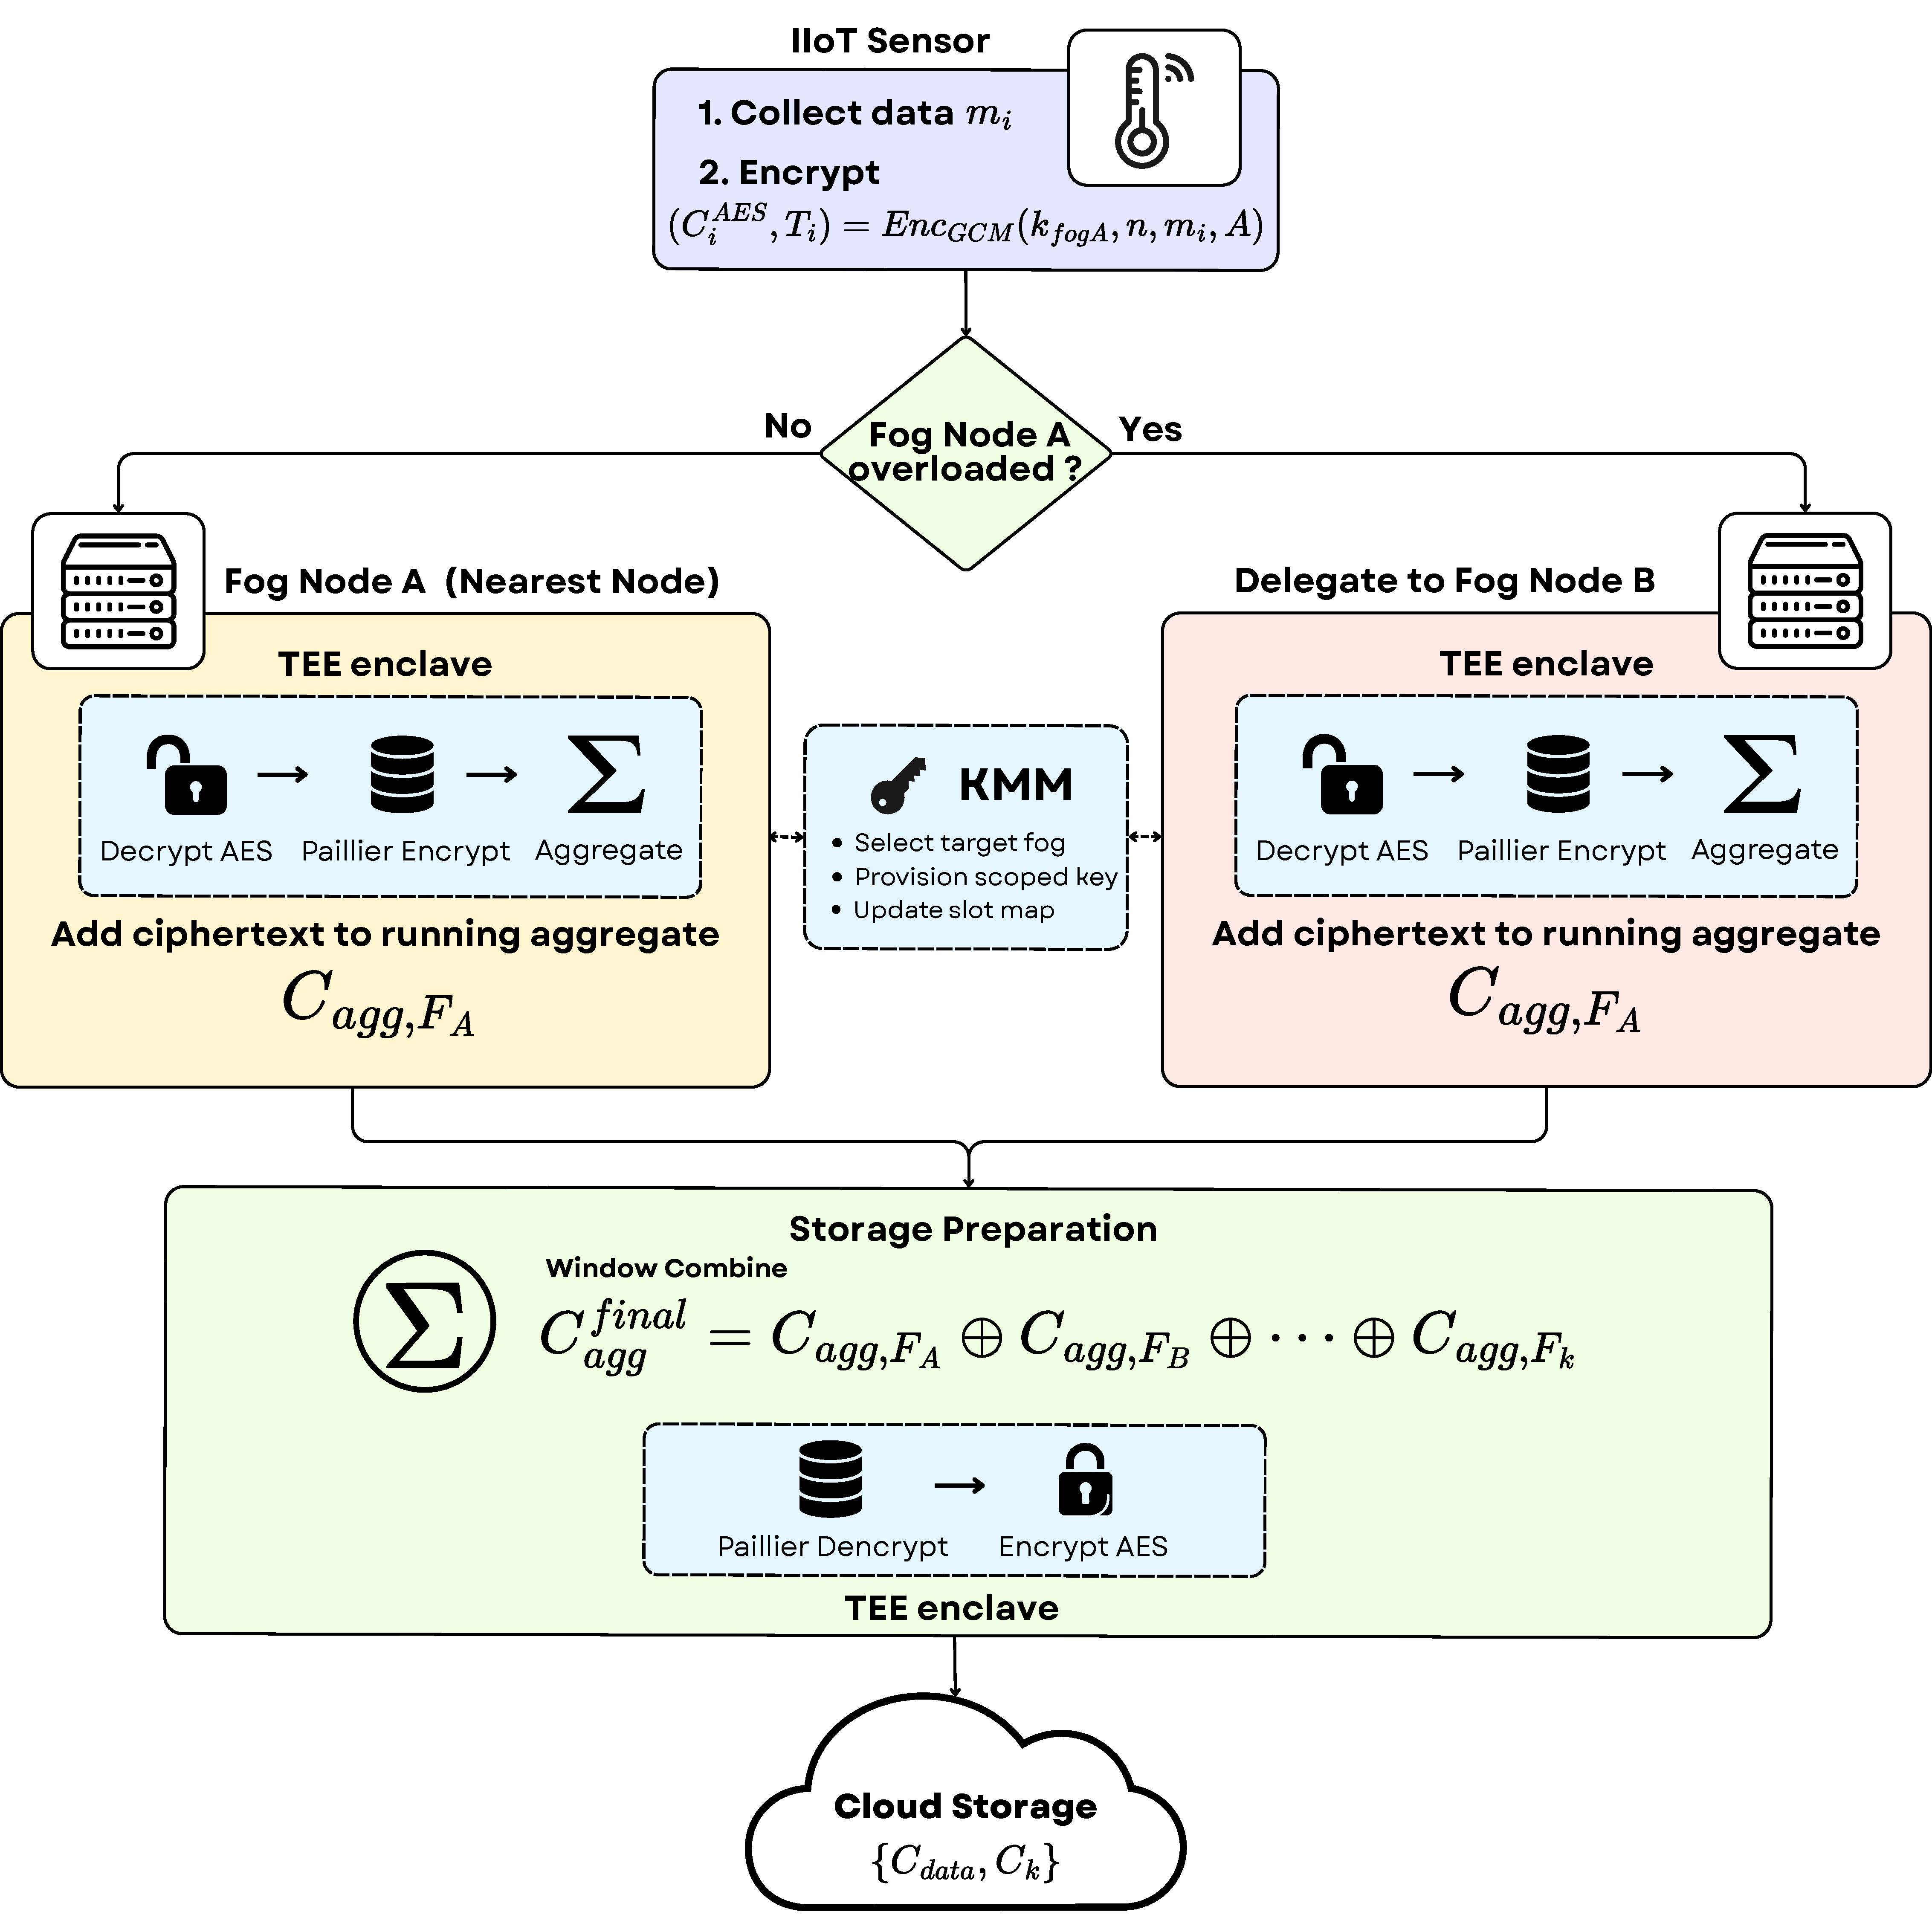
\includegraphics[width=1.0\linewidth]{../figures/flow_diagram.pdf}
        \caption{Proposed Secure IIoT Data Processing Framework with TEE-Enforced Key Transformation, Paillier Slot Aggregation, and KMM Window Combine}
        \label{fig:workflow}
    \end{figure}

    The overall secure data-processing workflow of the proposed framework is illustrated in Fig.~\ref{fig:workflow}.

    The process includes sensor-level AES-GCM encryption, fog-node tag verification, TEE-protected AES-to-Paillier conversion, Paillier slot aggregation, per-reading TEE delegation, KMM window combine, and secure AES-GCM cloud storage.

    Paillier partial homomorphic encryption is selected over fully homomorphic schemes such as CKKS and BFV because the target aggregation functions---sum, mean, and weighted sum---require only additive homomorphism. This design choice eliminates noise-budget management, rotation-key generation, and polynomial-degree tuning, reducing implementation complexity while maintaining IND-CPA security under the decisional composite residuosity assumption.

    \subsubsection{\textbf{Phase 1 Initialization}}

During initialization, the KMM generates fog-scoped AES keys,
Paillier keys, and the storage key. After successful
remote attestation, each fog enclave is provisioned only with its
own sealed fog-scoped key.

    \begin{equation}
    \forall F_i:\quad k_{fogI} \leftarrow KeyGen_{AES}()
    \end{equation}

    \begin{equation}
    (pk_P, sk_P) \leftarrow KeyGen_{Paillier}(2048)
    \end{equation}

    \begin{equation}
    k_{store} \leftarrow KeyGen_{AES}()
    \end{equation}

    \begin{equation}
    \forall F_i:\quad (ek_i, quote_i) \leftarrow TEE\_Attest(Enclave_i)
    \end{equation}

    \begin{equation}
    sealed\_kFogA = Seal(k_{fogA}, ek_A)
    \end{equation}

    The KMM retains $sk_P$ and $k_{store}$ and seals them for its own storage-preparation enclave:
    \begin{equation}
    \begin{aligned}
    sealed\_sk_P &= Seal(sk_P,\, ek_{SP}),\\
    sealed\_k_{store} &= Seal(k_{store},\, ek_{SP})
    \end{aligned}
    \end{equation}
    where $ek_{SP}$ is the sealing key of the dedicated storage-preparation enclave. These keys are never provisioned to fog-node enclaves.

    The KMM builds $slot\_map:sensor\_id\rightarrow fog\_node$, stores $fog\_node\rightarrow k_{fogI}$ for delegation provisioning, sets $W=T_g=500\,ms$, and initializes each fog node aggregate as
    \begin{equation}
    C_{agg,F_i} = Enc_P(pk_P,0).
    \end{equation}

    \subsubsection{\textbf{Phase 2 Sensor Data Encryption}}

    Each sensor encrypts its readings using AES-128-GCM under the fog-scoped key of its assigned fog node (four readings per window as stated in Section~\ref{sec:arch}). A sensor assigned to Fog~A encrypts only with $k_{fogA}$. Upon receiving a ciphertext, the fog node verifies the AES-GCM authentication tag using its provisioned fog-scoped key before passing the accepted ciphertext to the TEE enclave for processing. A single fog-node failure therefore affects 80 of 400 readings (20\% of window traffic) under an even sensor distribution.

    \begin{equation}
    (C_i^{AES},T_i) = Enc_{GCM}(k_{fogA}, n, m_i, A)
    \end{equation}

    \subsubsection{\textbf{Phase 3 Per-Reading Workload Check and Domain Conversion}}

    For every incoming ciphertext at Fog~A, delegation is decided immediately using the latest gossip value.
    \begin{equation}
    LastKnownWorkload(F_A) \geq \tau
    \end{equation}

    If the condition is false, Fog~A processes the reading inside its enclave and adds the Paillier ciphertext to its running aggregate in host memory.
    \begin{equation}
    m_i = Dec_{AES}(k_{fogA}, C_i^{AES})
    \end{equation}
    \begin{equation}
    C_i^P = Enc_P(pk_P, \lfloor m_i \cdot scale \rceil)
    \end{equation}
    \begin{equation}
    C_{agg,F_A} \leftarrow C_{agg,F_A} \oplus C_i^P
    \end{equation}

    If the condition is true, Fog~A zero-fills the vacated slot, notifies the KMM of the target fog node, and forwards the original AES ciphertext through the delegated processing path.
    \begin{equation}
    C_{zero} = Enc_P(pk_P,0)
    \end{equation}
    \begin{equation}
    C_{agg,F_A} \leftarrow C_{agg,F_A} \oplus C_{zero}
    \end{equation}

    \subsubsection{\textbf{Phase 4 TEE Delegation}}

    When delegation is triggered, Fog~A selects the target using the proposed CapacityScore (defined in Section~\ref{sec:lb}) over available non-primary candidates from its gossip table and notifies the KMM\@. Candidates with $Workload(F_j)<\tau$ are preferred, with fallback to all available non-primary nodes if every candidate is saturated. Fog~A does not transfer keys to Fog~B, and the sensor is not contacted.
    \begin{equation}
    F_{target}=\arg\max_{F_j\in\mathcal{C}} CapacityScore(F_j,\,t_{type})
    \end{equation}
    \begin{equation}
    Notify_{KMM}(s,F_A,F_{target})
    \end{equation}
    \begin{equation}
    Verify(quote_B)=true
    \end{equation}

    The KMM opens an attested channel to Enclave~B, provisions Fog~A's scoped key to Enclave~B for this delegation epoch, and updates $slot\_map:sensor~s\rightarrow Fog~B$.
    \begin{equation}
    sealed\_kFogA@B \leftarrow Provision_{KMM\rightarrow Enclave_B}(k_{fogA})
    \end{equation}
    \begin{equation}
    k_{fogA} \leftarrow Unseal(sealed\_kFogA@B,ek_B)
    \end{equation}

    Fog~B decrypts the delegated reading inside its enclave and accumulates the Paillier ciphertext in its own running aggregate. Delegated keys are revoked after the window closes, bounding the delegation exposure to one epoch.
    \begin{equation}
    m_s = Dec_{AES}(k_{fogA}, C_s^{AES})
    \end{equation}
    \begin{equation}
    C_s^P = Enc_P(pk_P, \lfloor m_s \cdot scale \rceil)
    \end{equation}
    \begin{equation}
    C_{agg,F_B} \leftarrow C_{agg,F_B} \oplus C_s^P
    \end{equation}
    \begin{equation}
    Revoke_{KMM}(k_{fogA}, Enclave_B)\quad \text{after } W
    \end{equation}

    \subsubsection{\textbf{Phase 4b ACK-Based Fault Detection with Gossip Redirect}}

    Gossip-only fault detection has a detection gap of $rT_g=3\times 500\,ms=1.5\,s$. During this interval, up to three aggregation windows may be affected before neighboring fog nodes identify the failed node. The proposed ACK-based mechanism reduces this gap to approximately $T_{ack}+T_{KMM}=100\,ms+50\,ms=150\,ms$ by allowing sensors to detect fog-node silence directly, notify the KMM, and redirect the encrypted reading using their local gossip table and the proposed CapacityScore (Eq.~\eqref{eq:capacityscore}) LS-default selector after delegated key provisioning.

    \paragraph{Operation.}
    Each time a sensor sends $C_i^{AES}$ to its assigned fog node, it starts a short ACK timer. The fog node returns a lightweight acknowledgement immediately after receiving and queuing the reading. If the ACK does not arrive within $T_{ack}$, the sensor performs the following local redirect procedure:

    \begin{itemize}
        \item The sensor consults its local gossip status table, which is maintained using $k\times 28$ bytes of RAM.
        \item It selects $F_{backup}=\arg\max_{F_j} CapacityScore(F_j,\,\text{LS})$ while excluding the silent fog node. Because raw sensor ciphertexts carry no task-type metadata, the LS weight configuration is used by default, as sensor readings must arrive within the active 500~ms aggregation window, satisfying the latency-sensitive routing criterion.
        \item It sends a small redirect notification to the KMM indicating that Fog~A is silent and Fog~B has been selected.
        \item The KMM provisions $sealed\_kFogA@B$ to Enclave~B through an attested channel, with expected provisioning latency of approximately $50\,ms$.
        \item It retransmits $C_i^{AES}$ directly to $F_{backup}$.
        \item Enclave~B decrypts with the provisioned $k_{fogA}$, so the blast radius is limited to Fog~A's sensor group and does not expose keys for other fog nodes.
    \end{itemize}

    \paragraph{Sensor gossip table memory cost.}
    Each fog-node status entry in the sensor's local table requires 28 bytes:

    \begin{table}[htbp]
    \caption{Sensor-Side Gossip Status Entry}
    \label{table:sensor-gossip-entry}
    \centering
    \resizebox{0.6\linewidth}{!}{
    \begin{tabular}{lc}
    \hline
    \textbf{Field} & \textbf{Size} \\
    \hline
    fog\_node\_id & 4 bytes \\
    workload & 4 bytes \\
    latency & 4 bytes \\
    queue\_length & 4 bytes \\
    timestamp & 8 bytes \\
    capacity\_score\_ls & 4 bytes \\
    \hline
    \textbf{Total per fog node} & \textbf{28 bytes} \\
    \hline
    \end{tabular}}
    \end{table}

    For $k=10$ fog nodes, the table consumes $10\times 28=280$ bytes. On a Cortex-M3 class IIoT sensor with 32~KB RAM, this is less than 1\% of available RAM and remains negligible for the proposed deployment model. No hardware upgrade is required.

    \paragraph{Sensor gossip table dissemination.}
    Each fog node rebroadcasts an HMAC-authenticated 280-byte gossip summary to its downstream sensors every $T_g=500\,\text{ms}$ ($\approx0.56\,\text{KB/s}$, negligible on 20~Mbps or higher links).

    \paragraph{Three-layer fault handling hierarchy.}
    The complete fault-handling system uses three layers, each covering failures that the previous layer cannot handle:

    \begin{table*}[htbp]
    \caption{Three-Layer Fault Handling Hierarchy}
    \label{table:fault-hierarchy}
    \centering
    \setlength{\tabcolsep}{3pt}
    \renewcommand{\arraystretch}{1.15}
    \begin{tabular}{@{}c>{\raggedright\arraybackslash}p{0.19\textwidth}>{\raggedright\arraybackslash}p{0.12\textwidth}>{\raggedright\arraybackslash}p{0.16\textwidth}>{\raggedright\arraybackslash}p{0.10\textwidth}>{\raggedright\arraybackslash}p{0.31\textwidth}@{}}
    \hline
    \textbf{Layer} & \textbf{Trigger} & \textbf{Who acts} & \textbf{Detection time} & \textbf{Data loss} & \textbf{Mechanism} \\
    \hline
    1 & Fog self-detects $Workload\geq\tau$ & Fog node & Immediate per reading & Zero & KMM-provisioned TEE delegation; sensor unaware \\
    2 & No ACK within $T_{ack}$ & Sensor and KMM & $T_{ack}+T_{KMM}\approx150\,ms$ & $\approx 150\,ms$ & Sensor notifies KMM, KMM provisions $k_{fogA}$ to Enclave~B, sensor retransmits $C_i^{AES}$ \\
    3 & $r=3$ missed gossip rounds & Fog neighbors and KMM & $rT_g=1.5\,s$ & $\approx 1.5\,s$ fallback & Neighbor detection and KMM reassignment \\
    \hline
    \end{tabular}
    \end{table*}

    \paragraph{Interaction with the Paillier slot protocol.}
    When Layer~2 triggers mid-window, the slot protocol handles redirected readings similarly to a normal delegation event after the ACK timeout. If Fog~A fails, its ACKs stop arriving at assigned sensors. Those sensors detect the silence within $T_{ack}=100\,ms$ and retransmit subsequent $C_i^{AES}$ values to Fog~B. However, because Fog~A is dead, it cannot zero-fill its own vacated slots in the current window. The KMM therefore handles the edge case at window close:

    \begin{itemize}
        \item The KMM detects that Fog~A did not submit $C_{agg,F_A}$ at window close.
        \item Fog~A's contribution is marked as zero for that window.
        \item The KMM combines the remaining fog-node aggregates as $C_{agg}^{final}=C_{agg,F_B}\oplus C_{agg,F_C}\oplus\cdots$.
        \item Readings already processed by Fog~A before failure are lost for that partial window if Fog~A never submitted its aggregate.
        \item Readings after the $T_{ack}$ redirect are captured at Fog~B.
    \end{itemize}

    The net result is partial-window recovery. Readings processed by Fog~A before failure are lost if Fog~A never submits its aggregate, while readings after ACK-timeout redirect are captured at Fog~B. Data loss is bounded to approximately the ACK redirect path rather than the full $1.5\,s$ gossip fallback interval.

    \subsubsection{\textbf{Phase 4c Window Close and KMM Combine}}

    At every $W=500\,ms$ window close, each fog node sends one aggregate ciphertext to the KMM. The KMM performs only homomorphic addition and does not decrypt.
    \begin{equation}
    C_{agg}^{final} = C_{agg,F_1} \oplus C_{agg,F_2} \oplus \cdots \oplus C_{agg,F_k}
    \end{equation}

    The KMM then sends $C_{agg}^{final}$ to an attested enclave for storage preparation and each fog node resets its aggregate to $Enc_P(pk_P,0)$ for the next window.

    \subsubsection{\textbf{Phase 5 Secure Storage Preparation}}

    The KMM forwards $C_{agg}^{final}$ to the dedicated storage-preparation enclave, the sole holder of $sk_P$ and $k_{store}$. Inside this enclave, the Paillier aggregate is decrypted and re-encrypted for compact cloud storage; both keys and the aggregate plaintext never leave enclave memory.
    \begin{equation}
    D_{agg} = Dec_P(sk_P, C_{agg}^{final})
    \end{equation}
    \begin{equation}
    C_{data} = Enc_{AES}(k_{store},\, \{D_{agg},\, \mathrm{metadata}\})
    \end{equation}
    \subsubsection{\textbf{Phase 6 Cloud Storage}}

    The cloud stores only the AES-encrypted aggregate.
    \begin{equation}
    Cloud \leftarrow C_{data}
    \end{equation}

    \subsection{Trust Model: Fog-Scoped Key Isolation}

    The original single-global-key design creates a broad compromise domain because one broken fog enclave can expose every sensor stream. The proposed design replaces that model with fog-scoped keys, so each fog node holds only the AES key for its assigned sensor group. The KMM remains the trust anchor and provisions delegated keys only to attested enclaves for bounded delegation epochs.

    \begin{table*}[htbp]
    \caption{Compromise Blast Radius Across Key-Provisioning Designs}
    \label{table:trust-model}
    \centering
    \begingroup
    \setlength{\tabcolsep}{3pt}
    \renewcommand{\arraystretch}{1.15}
    \begin{tabular}{@{}>{\raggedright\arraybackslash}p{0.18\textwidth}>{\raggedright\arraybackslash}p{0.12\textwidth}>{\raggedright\arraybackslash}p{0.12\textwidth}>{\raggedright\arraybackslash}p{0.17\textwidth}>{\raggedright\arraybackslash}p{0.33\textwidth}@{}}
    \hline
    \textbf{Compromise scenario} & \textbf{Global AES key} & \textbf{All-at-init keys} & \textbf{Fog-scoped $k_{fogI}$} & \textbf{Reason} \\
    \hline
    Fog host OS reads memory & None & None & None & TEE blocks host access to enclave memory \\
    Fog TEE enclave physically broken & All sensors & All sensors & Only that fog node's sensor group & Fog-scoped keys bound the exposed decryption key \\
    KMM compromised & All sensors & All sensors & All fog groups & KMM is the system trust anchor \\
    Network eavesdropping & None & None & None & Transmissions remain AES-, Paillier-, or attested-channel protected \\
    Fog B compromised during delegation & All sensors & All sensors & Fog A and Fog B groups only & KMM provisions only $k_{fogA}$ to Enclave~B \\
    \hline
    \end{tabular}
    \endgroup
    \end{table*}

    The Key Management Module is the system trust anchor. It is assumed to be deployed in a hardened, high-availability environment separate from fog infrastructure. Compromise of the KMM exposes all fog-scoped keys. Compromise of a single fog node's TEE enclave, which requires physical hardware attack beyond the standard honest-but-curious fog-host threat model, exposes only that node's assigned sensor group's decryption key for the current delegation epoch. Historical data already stored as AES ciphertexts in the cloud remains protected by $k_{store}$, held exclusively in the KMM's storage-preparation enclave.

    After each delegation window closes, the KMM revokes $k_{fogA}$ from Enclave~B. Enclave~B holds the delegated key only for the duration of one $500\,ms$ window, limiting the exposure period even if Enclave~B is compromised later.

    The load-balancing and fault-tolerance mechanisms share the same per-reading KMM-provisioned reassignment infrastructure. Load balancing is triggered when $LastKnownWorkload(F_i) \geq \tau$ for an incoming reading. Fault tolerance is triggered either by sensor ACK timeout or by $r$ consecutive missed gossip rounds; in both cases, the KMM provisions only the failed or overloaded fog node's scoped key to the receiving enclave. The current failure window may contain a partial aggregate if the failed node did not deliver $C_{agg,F_i}$ to the KMM before failure.
    \subsubsection{\textbf{Paillier Slot Mechanics and Storage Reduction}}

    The slot protocol preserves aggregate correctness when delegation occurs mid-window. Under normal operation, Fog~A accumulates all readings assigned to it as $C_{agg,F_A}=C_1^P\oplus\cdots\oplus C_n^P$. If sensor $s$ is delegated during the same window, Fog~A adds $C_{zero}=Enc_P(pk_P,0)$ for the vacated slot while Fog~B adds the delegated reading $C_s^P$ to $C_{agg,F_B}$. At window close, KMM computes $C_{agg}^{final}=C_{agg,F_A}\oplus C_{agg,F_B}\oplus\cdots$, producing the same sum as if no delegation had occurred.

    Paillier slot aggregation reduces the number of ciphertexts stored per window from $n$ sensor ciphertexts to one aggregate ciphertext. For $n=100$ sensors, this changes the per-window storage pattern from 100 individual readings to a single Paillier aggregate before compact AES storage preparation. The supported aggregation functions are sum, mean, and weighted sum; variance, standard deviation, threshold count, maximum, and minimum require multiplication or comparison and are outside the Paillier-only scope.

    \paragraph{IND-CPA security of vacated slots.}
    Each zero-fill ciphertext $C_{zero}=\text{Enc}_P(pk_P,0)$ is generated with a freshly sampled random coin. Under the Decisional Composite Residuosity (DCR) assumption that underlies Paillier IND-CPA security, $C_{zero}$ is computationally indistinguishable from a real reading ciphertext $C_i^P$. An adversary observing the host-memory aggregate $C_{agg,F_A}$ therefore cannot determine which slots were vacated by delegation without access to $sk_P$, which remains sealed inside the storage-preparation enclave and is never provisioned to fog-node enclaves.

    \subsection{Load Balancing Mechanism}
    \label{sec:lb}
    \subsubsection{Workload Monitoring and Overload Detection}

    Each fog node continuously monitors its system resources to determine its processing capability. Before aggregation, each raw metric is normalized to the range $[0,1]$ as

    \begin{equation}
    \begin{aligned}
    \widehat{CPU}_i &= \min\!\left(\frac{CPU_i^{used}}{CPU_i^{cap}},1\right),\\
    \widehat{RAM}_i &= \min\!\left(\frac{RAM_i^{used}}{RAM_i^{cap}},1\right),\\
    \widehat{BW}_i &= \min\!\left(\frac{BW_i^{used}}{BW_i^{cap}},1\right)
    \end{aligned}
    \end{equation}

    The workload of fog node $F_i$ is then computed as
    \begin{equation}
    Workload(F_i) = 0.5\,\widehat{CPU}_i + 0.3\,\widehat{RAM}_i + 0.2\,\widehat{BW}_i
    \label{eq:workload-definition}
    \end{equation}

    where $CPU_i^{used}$, $RAM_i^{used}$, and $BW_i^{used}$ denote current usage and $CPU_i^{cap}$, $RAM_i^{cap}$, and $BW_i^{cap}$ denote node capacity for each resource. The weights $0.5$, $0.3$, and $0.2$ reflect aggregate resource pressure across the full mix of task types: CPU dominates for compute-heavy tasks such as FFT-based spectral analysis, while bandwidth becomes the binding constraint for latency-sensitive sensor-reading tasks. This formula captures the composite overload signal used to trigger delegation; per-task routing is handled separately by the $compat$ term in the CapacityScore (Eq.~\eqref{eq:capacityscore}), which assigns an 0.80 bandwidth weight for latency-sensitive tasks and a $\phi_j^2$-penalised CPU weight for heavy-processing tasks.

    In this framework, $\tau = 0.8$, indicating that the node is operating at 80\% or higher \emph{normalized} composite resource utilization. This value balances responsiveness and stability: a threshold below $0.7$ risks unnecessary delegation during transient load spikes, while a threshold above $0.85$ leaves insufficient headroom for the additional cryptographic operations required during secure handoff.
    \begin{equation}
    Workload(F_i) \geq \tau
    \end{equation}

    To maintain awareness of the system state, fog nodes exchange status information through a gossip-based communication protocol. At every gossip interval $T_g=500\,ms$, each fog node randomly selects $k=3$ neighboring nodes and sends a lightweight status message containing its current workload, queue length, network latency estimate, and two pre-computed compatibility scores: $compat_{LS}$ and $compat_{HP}$, evaluated locally using the node's live $\widehat{CPU}$, $\widehat{RAM}$, and $\widehat{BW}$ values before broadcast. Carrying pre-computed compat scores rather than raw resource fractions keeps the gossip payload compact while giving receiving nodes all the information needed to evaluate the full CapacityScore (Eq.~\eqref{eq:capacityscore}) without direct access to the sender's internal state.

    Upon receiving a gossip message, the neighbor updates its local status table and may further propagate the information to other nodes in subsequent gossip rounds. Through this decentralized information exchange, fog nodes gradually build and maintain a $LastKnownWorkload$ table containing the most recent system state of nearby nodes. Gossip updates this table every $T_g$, while delegation reads the table on every incoming sensor reading; delegation therefore does not wait for either a gossip round or a window boundary.

    \subsubsection{Load Redistribution and Fog Node Selection}

    When $LastKnownWorkload(F_i)\geq\tau$ for an incoming reading, the fog node initiates a load redistribution procedure for that reading. Using the status information obtained from the gossip protocol, the overloaded node evaluates candidate fog nodes and selects the most suitable destination for task delegation. The selection is based on a \textit{CapacityScore} (S6), which jointly reflects a node's current load, network latency, queue occupancy, and structural compatibility with the incoming task type.

    The CapacityScore of candidate fog node $F_j$ for a task of type $t_{type}$ is computed as

    \begin{equation}
    \begin{aligned}
    CapacityScore(F_j,t_{type}) =\;& w_1(1-Workload(F_j)) \\
    &+ w_2(1-\ell_j) \\
    &+ w_3(1-q_j) \\
    &+ w_4\cdot compat(F_j,t_{type})
    \end{aligned}
    \label{eq:capacityscore}
    \end{equation}

    where $Workload(F_j)$ is the normalized workload from Eq.~\eqref{eq:workload-definition}. For dimensional consistency, latency and queue occupancy are normalized to $[0,1]$ as

    \begin{equation}
    \begin{aligned}
    \ell_j &= \min\!\left(\frac{lat_j}{lat_j^{cap}},1\right),\\
    q_j &\in [0,1] \text{ (gossip-reported occupancy fraction)}
    \end{aligned}
    \label{eq:e5-normalized-latency-queue}
    \end{equation}

    where $lat_j$ is the observed round-trip latency of node $F_j$, $lat_j^{cap}$ is its configured latency ceiling, and $q_j \in [0,1]$ is the queue occupancy fraction reported by the gossip protocol. The compatibility term $compat(F_j,t_{type})\in[0,1]$ captures the structural suitability of a node for the task type. For Latency-Sensitive (LS) tasks, which are bandwidth-dominant, it weights available bandwidth heavily:

    \begin{equation}
    \begin{aligned}
    compat_{LS}(F_j) =\;& 0.10(1-\widehat{CPU}_j) \\
    &+ 0.10(1-\widehat{RAM}_j) \\
    &+ 0.80(1-\widehat{BW}_j)
    \end{aligned}
    \end{equation}

    For Heavy Processing (HP) tasks, which require fast CPU cores, a node-speed factor $\phi_j^2$ penalises structurally slow nodes regardless of current load:

    \begin{equation}
    \begin{aligned}
    compat_{HP}(F_j) =\;& 0.60\,\phi_j^2(1-\widehat{CPU}_j)\\
    &+ 0.30(1-\widehat{RAM}_j) \\
    &+ 0.10(1-\widehat{BW}_j)
    \end{aligned}
    \end{equation}

    The node-speed factor $\phi_j \in (0,1]$ reflects the relative processing speed of each fog node, and execution time is modeled as $T_{exec}=base\_time/\phi_j$. The $\phi_j^2$ multiplier penalises structurally slow nodes: a node with half the reference speed contributes at most one quarter of the maximum HP CPU-compatibility score, steering compute-heavy tasks away from nodes that cannot meet their execution deadlines regardless of their current load.
    The parameters $w_1$, $w_2$, $w_3$, and $w_4$ are dynamic weights that adapt based on the incoming task type, where

    \begin{equation}
    w_1 + w_2 + w_3 + w_4 = 1
    \end{equation}

    All score components are dimensionless in $[0,1]$ before inversion, so the CapacityScore remains comparable across heterogeneous fog nodes. The fog node with the highest CapacityScore is selected as the delegation destination:

    \begin{equation}
    F_{target} = \arg\max_{F_j \in N_i} CapacityScore(F_j,\,t_{type})
    \end{equation}

    where $N_i$ represents the set of neighboring fog nodes discovered through the gossip-based status exchange, excluding failed nodes and the primary node itself. The proposed method first restricts $N_i$ to nodes with $Workload(F_j)<\tau$ and falls back to all available non-primary nodes only if no under-threshold candidate exists.


    \subsubsection{Task-Aware Dynamic Weight Assignment}

    Rather than applying fixed weights uniformly, the CapacityScore adapts based on the incoming task type. Each task submitted by an IoT device carries a \textit{max\_delay} metadata field that classifies the task into a routing-priority tier, selecting the weight configuration used in the CapacityScore formula. This field is a classification hint, not an end-to-end deadline on the fixed $W=500\,ms$ aggregation window. The fog node uses this value to classify the task into one of two types.

    \begin{table}[htbp]
    \caption{Task Classification Based on Delay Requirement}
    \label{table:task-classification}
    \centering
    \begingroup
    \setlength{\tabcolsep}{3pt}
    \renewcommand{\arraystretch}{1.15}
    \begin{tabular}{@{}>{\raggedright\arraybackslash}p{0.28\linewidth}>{\raggedright\arraybackslash}p{0.25\linewidth}>{\raggedright\arraybackslash}p{0.37\linewidth}@{}}
    \hline
    \textbf{Task Type} & \textbf{Condition} & \textbf{Example Applications} \\
    \hline
    Latency-Sensitive & $max\_delay \leq 100\,ms$ & Real-time health monitoring, industrial control systems \\
    Heavy Processing & $max\_delay > 100\,ms$ & Video frame analysis, compression tasks \\
    \hline
    \end{tabular}
    \endgroup
    \end{table}

    Once the task type is determined, the fog node selects the corresponding weight configuration for the CapacityScore computation:

    \begin{equation}
    (w_1, w_2, w_3, w_4) =
    \begin{cases}
    (0.10,\; 0.35,\; 0.10,\; 0.45), &
    \substack{\text{Latency-Sensitive}\\\text{(LS)}} \\
    (0.15,\; 0.30,\; 0.10,\; 0.45), &
    \substack{\text{Heavy Processing}\\\text{(HP)}}
    \end{cases}
    \end{equation}

    In both configurations, the compatibility weight $w_4 = 0.45$ is the dominant term, ensuring that structural node suitability drives the selection decision beyond raw load conditions. For LS tasks, $w_2 = 0.35$ gives secondary priority to network latency, since these tasks are delay-critical. For HP tasks, $w_2 = 0.30$ and the $\phi_j^2$ factor inside $compat_{HP}$ applies a strong structural penalty to slow nodes, steering compute-heavy tasks away from nodes that cannot meet their execution deadlines. Raw sensor ciphertexts routed during fault recovery (Layers 2 and 3) use the LS configuration by default, as explained in Section~\ref{sec:lb}.

    Because gossip refreshes $LastKnownWorkload$ every $T_g$ while delegation is checked on every incoming ciphertext, a reading can be delegated at any time within $t\in[0,W]$ rather than waiting for the next window close.

\begin{algorithm}
\caption{Runtime TEE-Assisted Paillier Slot Aggregation with Load-Balanced Delegation}
\label{alg:runtime_delegation}
\begin{algorithmic}[1]
\REQUIRE Initialized fog nodes $\{F_1,\ldots,F_k\}$, fog-scoped keys $k_{fogI}$, Paillier public key $pk_P$, aggregation window $W$, workload threshold $\tau$, and initialized aggregates $C_{agg,F_i}=Enc_P(pk_P,0)$
\REQUIRE Latest gossip tables containing $LastKnownWorkload$, $LastKnownQueue$, $LastKnownLatency$, $LastKnownCompatLS$, and $LastKnownCompatHP$
\ENSURE Updated per-fog Paillier aggregates $\{C_{agg,F_1},\ldots,C_{agg,F_k}\}$ for the current window

\FOR{each sensor reading $C_i^{AES}$ assigned to fog node $F_A$ during window $W$}
    \IF{$F_A$ is unavailable \OR $LastKnownWorkload(F_A) \geq \tau$}
        \STATE Classify $task\_type \in \{LS,HP\}$ from task metadata
        \STATE Build candidate set:
        \[
        \begin{aligned}
        \mathcal{C}=\{F_j: & F_j\neq F_A,\;F_j\ \text{available},\\
        & LastKnownWorkload(F_j)<\tau\}
        \end{aligned}
        \]
        \IF{$\mathcal{C}=\emptyset$}
            \STATE $\mathcal{C}=\{F_j:F_j\neq F_A,\;F_j\ \text{available}\}$
            \COMMENT{Fallback when all candidates are saturated}
        \ENDIF

        \STATE Select target fog node:
        \[
        F_{target}=\arg\max_{F_j\in\mathcal{C}} CapacityScore(F_j,task\_type)
        \]

        \IF{$F_A$ is still alive}
            \STATE $C_{zero}=Enc_P(pk_P,0)$
            \STATE $C_{agg,F_A}\leftarrow C_{agg,F_A}\oplus C_{zero}$
            \COMMENT{Preserve vacated slot correctness}
        \ENDIF

        \STATE Notify KMM that sensor $s$ is delegated from $F_A$ to $F_{target}$
        \STATE Forward $C_i^{AES}$ to $F_{target}$
        \STATE KMM verifies $quote_{F_{target}}$
        \STATE KMM provisions $sealed\_kFogA@F_{target}$ to $Enclave_{F_{target}}$
        \STATE KMM updates $slot\_map:s\rightarrow F_{target}$

        \STATE $k_{fogA}=Unseal(sealed\_kFogA@F_{target},ek_{F_{target}})$ inside $Enclave_{F_{target}}$
        \STATE $m_i=Dec_{AES}(k_{fogA},C_i^{AES})$ inside $Enclave_{F_{target}}$
        \STATE $C_i^P=Enc_P(pk_P,\lfloor m_i\cdot scale\rceil)$
        \STATE $C_{agg,F_{target}}\leftarrow C_{agg,F_{target}}\oplus C_i^P$

    \ELSE
        \STATE $m_i=Dec_{AES}(k_{fogA},C_i^{AES})$ inside $Enclave_A$
        \STATE $C_i^P=Enc_P(pk_P,\lfloor m_i\cdot scale\rceil)$
        \STATE $C_{agg,F_A}\leftarrow C_{agg,F_A}\oplus C_i^P$
    \ENDIF
\ENDFOR

\end{algorithmic}
\end{algorithm}

    \subsection{Fault Tolerance Mechanism}
    Fog node failures are modeled using a Poisson process~\cite{abdelbasset2019fault}. The probability of $p$ failures in interval $T$ is

    \begin{equation}
    P(p) = \frac{(\mu T)^p e^{-\mu T}}{p!}
    \end{equation}

    where $\mu$ is the average failure rate and $T$ the observation interval. The probability of at least one failure is

    \begin{equation}
    P(p \geq 1) = 1 - P(0) = 1 - e^{-\mu T}
    \end{equation}

    For gossip-based failure detection, the observation window is $T = rT_g$, where $r$ is the consecutive-miss threshold and $T_g$ is the gossip period. Substituting gives the probability that at least one failure \emph{arrives} within the gossip observation window:

    \begin{equation}
    P(p \geq 1 \mid T = rT_g) = 1 - e^{-\mu r T_g}
    \end{equation}

    This is a failure-arrival model, not a detector model. The deterministic worst-case detection delay of the gossip mechanism is $rT_g$; smaller $T_g$ improves detection timeliness at the cost of higher gossip traffic. The arrival probability above can be used to select $T_g$: if a deployment requires that any failure arrives within the observation window with probability at most $\beta$, then $T_g$ should satisfy

    \begin{equation}
    T_g \leq \frac{-\ln(1-\beta)}{\mu r}
    \end{equation}

    For $\beta = 0.95$ this gives $T_g \leq \ln(20)/(\mu r)$. In the proposed system, the gossip parameters $r=3$ and $T_g=500\,\text{ms}$ are chosen to bound the worst-case detection delay to $rT_g = 1.5\,\text{s}$; the ACK-redirect path (Phase 4b) reduces effective recovery latency to $150\,\text{ms}$ for the common single-node failure case.

    The proposed framework uses gossip-based failure detection~\cite{demers1988epidemic}: each fog node broadcasts its status every $T_g=500\,ms$ to $k=3$ randomly selected neighbors and is declared unavailable after $r=3$ consecutive missed rounds ($rT_g=1.5\,s$ worst-case detection). In the event of a network partition, the partitioned node initiates local failover by promoting the highest-scoring known neighbor using the most recently cached CapacityScore (LS-default configuration).

    Once a failure is detected, recovery proceeds through either sensor-side ACK redirect or gossip-triggered reassignment, both using the S6 LS-default selector. In both cases, sealed key material is never exposed to the fog host OS. If the failed node did not deliver $C_{agg,F_i}$ before failure, that window is treated as a partial aggregate; subsequent windows are handled by the promoted target node.

\begin{algorithm}
\caption{Fault Recovery, Window Combine, and Secure Storage}
\label{alg:fault_window_storage}
\begin{algorithmic}[1]
\REQUIRE Gossip table, $T_g$, $r$, $T_{ack}$, $\tau$, aggregates $\{C_{agg,F_i}\}$, $sk_P$, $k_{store}$
\ENSURE Cloud stores $C_{data}$

\STATE Each fog node computes $compat_{LS}$ and $compat_{HP}$ locally from live $\widehat{CPU}$, $\widehat{RAM}$, $\widehat{BW}$
\STATE \parbox[t]{0.88\linewidth}{Each fog node gossips $\{workload, queue, latency, \phi,$\\
$compat_{LS}, compat_{HP}, timestamp\}$ every $T_g$}
\STATE Update $LastKnownWorkload$, $LastKnownQueue$, $LastKnownLatency$, $LastKnownCompatLS$, and $LastKnownCompatHP$

\IF{$miss_{gossip}(F_A)\geq r$}
    \STATE \[\begin{aligned}
        \mathcal{C}\;\leftarrow\{F_j: & F_j\neq F_A,\;F_j\ \text{available},\\
        & LastKnownWorkload(F_j)<\tau\}
        \end{aligned}
        \]
    \IF{$\mathcal{C}=\emptyset$}
        \STATE $\mathcal{C}\leftarrow \{F_j:F_j\neq F_A,\;F_j\ \text{available}\}$
    \ENDIF
    \STATE \parbox[t]{0.88\linewidth}{$F_{target}\leftarrow \arg\max_{F_j\in\mathcal{C}}$\\
    $LastKnownCapacityScore_{LS}(F_j)$}
    \STATE Mark $F_A$ unavailable and redirect its remaining sensors to $F_{target}$
    \STATE KMM provisions $sealed\_kFogA@F_{target}$ to $Enclave_{F_{target}}$
    \STATE KMM updates affected $slot\_map$ entries
\ENDIF

\IF{sensor $s$ misses ACK from $F_A$ within $T_{ack}$}
    \STATE \parbox[t]{0.88\linewidth}{$F_{backup}\leftarrow \arg\max_{F_j\neq F_A}$\\
    $LocalGossipCapScore(F_j)$}
    \STATE Sensor notifies KMM and retransmits $C_i^{AES}$ to $F_{backup}$
    \STATE KMM provisions $sealed\_kFogA@F_{backup}$ to $Enclave_{F_{backup}}$
    \STATE $Enclave_{F_{backup}}$ decrypts $C_i^{AES}$, converts it to $C_i^P$, and updates $C_{agg,F_{backup}}$
\ENDIF

\STATE At window close, each available fog node sends $C_{agg,F_i}$ to KMM
\STATE Missing fog-node aggregates are treated as zero for the current window
\STATE KMM computes $C_{agg}^{final}\leftarrow C_{agg,F_1}\oplus\cdots\oplus C_{agg,F_k}$
\STATE Reset each $C_{agg,F_i}\leftarrow Enc_P(pk_P,0)$
\STATE Revoke delegated fog-scoped keys from receiving enclaves

\STATE $D_{agg}\leftarrow Dec_P(sk_P,C_{agg}^{final})$ inside storage-preparation enclave
\STATE $C_{data}\leftarrow Enc_{AES}(k_{store},\{D_{agg},metadata\})$
\STATE Store $C_{data}$ in cloud

\end{algorithmic}
\end{algorithm}

    \section{Performance Evaluation}
    \label{sec:evaluation}

    \subsection{Experimental Setup}
    \label{sec:eval-setup}

    All experiments are implemented in Python~3.13 using the \texttt{phe}~1.5.0 Paillier library with 2048-bit RSA moduli and a fixed-point scaling factor of $scale=1000$. The simulation environment consists of five heterogeneous fog nodes $F_1$--$F_5$ whose hardware profiles are summarized in Table~\ref{table:fog-nodes}. The nodes range from a weak single-core node ($F_3$: 1~CPU core, 2~GB RAM, 20~Mbps) to strong quad-core nodes ($F_1$, $F_5$: 4~CPU cores, 8~GB RAM, 100~Mbps), each serving 20 sensors for a total of 100 sensors. The overload threshold is $\tau=0.8$, the aggregation window is $W=T_g=500\,\text{ms}$, the sensor ACK timeout is $T_{ack}=100\,\text{ms}$, and the KMM provisioning latency is $T_{KMM}=50\,\text{ms}$.

    \begin{table}[htbp]
    \caption{Fog Node Hardware Profiles Used in Simulation}
    \label{table:fog-nodes}
    \centering
    \resizebox{1.0\linewidth}{!}{
    \begin{tabular}{llrrrrr}
    \hline
    \textbf{Node} & \textbf{Class} & \textbf{CPU Cores} & \textbf{RAM (GB)} & \textbf{BW (Mbps)} & \textbf{Sensors} & $\boldsymbol{\phi_j}$ \\
    \hline
    $F_1$ & Strong      & 4 & 8 & 100 & 20 & 1.00 \\
    $F_2$ & Medium      & 2 & 4 &  50 & 20 & 0.50 \\
    $F_3$ & Weak        & 1 & 2 &  20 & 20 & 0.25 \\
    $F_4$ & Medium-Fast & 2 & 4 &  80 & 20 & 0.50 \\
    $F_5$ & Strong      & 4 & 8 & 100 & 20 & 1.00 \\
    \hline
    \end{tabular}}
    \begin{flushleft}
    \footnotesize $\phi_j = \text{CPU cores}_j \;/\; \max_j(\text{CPU cores})$; normalized to the strongest node (4~cores).
    \end{flushleft}
    \end{table}

    The TEE layer is emulated using OP-TEE running on QEMU (ARM TrustZone emulation). Enclave operations---AES-GCM decryption, Paillier encryption, and key unsealing---are modeled as OP-TEE Trusted Applications executing within the secure world. The \texttt{sgx\_enclave\_process} function in the prototype implements these operations using the OP-TEE QEMU environment; no actual SGX hardware boundary, SGX sealing-key derivation, or SGX remote attestation exchange is present in the simulation. Measured latencies in E2 are host-reference OP-TEE QEMU values and should not be interpreted as physical hardware timings. The architectural design is expressed using generic TEE terminology (sealing, remote attestation, enclave quotes); Intel SGX is used as the reference implementation because Intel SGX and ARM TrustZone/OP-TEE provide equivalent security primitives under the same TEE trust model. Validation on physical SGX or TrustZone hardware is reserved for future work.

    Experiments E1--E2, E3a--E3b, and E4 evaluate the prototype implementation using a calibrated 2048-bit host-reference Paillier benchmark (\texttt{host\_reference\_2048\_no\_ta} mode). E5 is a simulation study averaged over 20 seeds $\{42,\ldots,61\}$ with 95\% CI. E6, E7, and E8 are analytical models. All results are organized into three thematic groups below.

    \subsection{Storage and Latency Efficiency}
    \label{sec:eval-storage-latency}

    \textbf{Storage reduction (E1).} For sensor counts $n\in\{10,50,100,200,500,1000\}$, cloud storage is compared under four schemes: plaintext ($n\times8$~bytes), AES-GCM per-reading ($n\times36$~bytes), Paillier without aggregation ($n\times512$~bytes), and the proposed method (one fixed-size $C_{data}$ per window). As shown in Fig.~\ref{fig:e1-storage}, the proposed method stores exactly one ciphertext per window regardless of $n$, achieving $100\times$ byte reduction over AES-GCM per-reading at $n=100$ and $1000\times$ at $n=1000$. Paillier slot aggregation thus reduces cloud storage from $O(n)$ to $O(1)$.

    \begin{figure}[htbp]
    \centering
    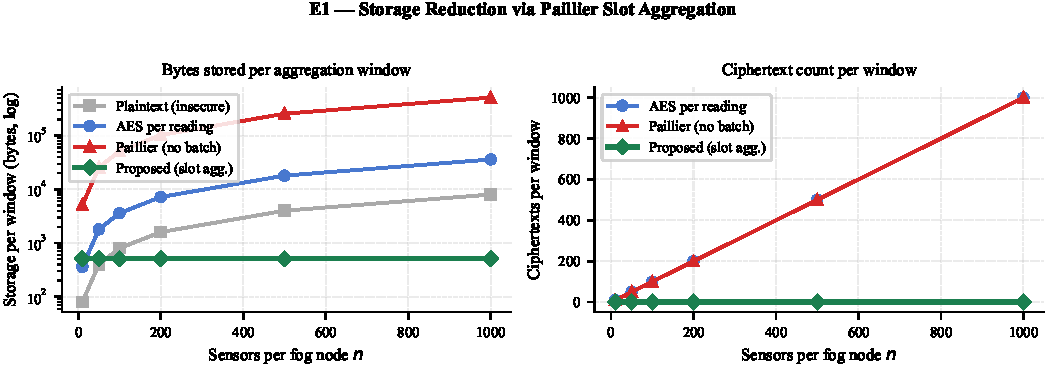
\includegraphics[width=1.0\linewidth]{../figures/exp1_storage.pdf}
    \caption{Storage comparison across schemes vs sensor count $n$. Upper panel: total bytes; lower panel: ciphertext count. The proposed method stores one ciphertext per window for all $n$.}
    \label{fig:e1-storage}
    \end{figure}

    \textbf{Aggregation latency (E2).} Using calibrated 2048-bit Paillier timings, the proposed pipeline requires $444.128$~ms in total: $227.537$~ms for fog TA conversion, $1.474$~ms for host aggregation and KMM window combine, and $215.117$~ms for storage TA preparation (Fig.~\ref{fig:e2-latency}). The total is within the 500~ms aggregation window; fog conversion and storage preparation dominate, while the KMM combine step contributes only $\approx6$~ms for the five-node deployment evaluated here (scaling linearly with $k$; see E4). These timings are host-reference values from the OP-TEE QEMU simulation described in Section~\ref{sec:eval-setup} and should not be interpreted as physical hardware timings. The discrepancy between this $444.128$~ms measured figure and the $399$~ms hardware-target estimate below reflects the absence of AES-NI acceleration and a hardware Paillier co-processor in the QEMU environment.

    \textbf{Claim (Latency Budget):} Under the hardware-target analytical model, the proposed pipeline completes within $W=500$~ms in non-delegation windows ($399$~ms). When delegation is triggered, the window budget is exceeded by exactly $T_{KMM}\approx150$~ms for TEE key provisioning---an overhead that is bounded, one-time per delegation event, and predictable at scheduling time. In the 20-window evaluation schedule, the 12 non-delegation windows (W1--5, W14--17, and the normal-load portions of W11--13) complete at $399$~ms. The 8 delegation-burst windows (W6--10, W18--20) each incur this fixed $150$~ms overhead; deployments serving burst phases should provision a $650$~ms extended window or absorb the overhead through capacity headroom. Fig.~\ref{fig:e7-pipeline} shows the per-window breakdown across all 20 windows.

    \begin{figure}[htbp]
    \centering
    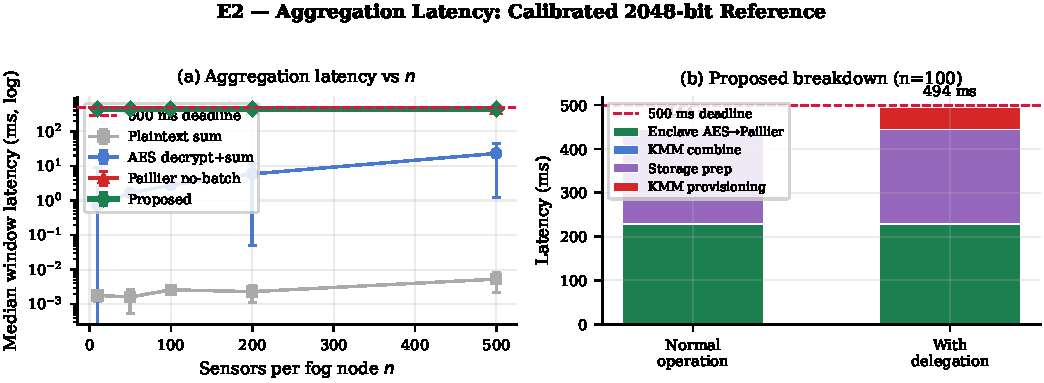
\includegraphics[width=1.0\linewidth]{../figures/exp2_latency.pdf}
    \caption{Aggregation latency vs sensor count $n$ with calibrated 2048-bit host-reference Paillier timings. The dashed line marks 500~ms. The right panel shows the component breakdown.}
    \label{fig:e2-latency}
    \end{figure}

    \begin{figure}[htbp]
    \centering
    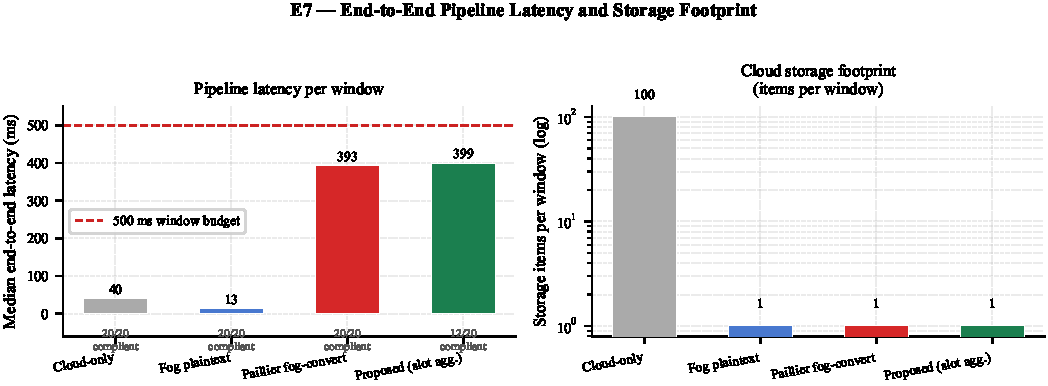
\includegraphics[width=1.0\linewidth]{../figures/exp7_pipeline.pdf}
    \caption{Analytical pipeline latency (left) and per-window storage items (right) across 20 windows under hardware-target constants. The dashed line marks 500~ms; delegation windows incur a bounded $T_{KMM}=150$~ms overhead above the non-delegation baseline of 399~ms.}
    \label{fig:e7-pipeline}
    \end{figure}

    Table~\ref{tab:e7-baselines} places the proposed pipeline within the
    landscape of fog architectures by comparing per-window cloud storage
    and latency sources across four representative methods under identical
    hardware-target assumptions ($n=100$ sensors). All latency estimates
    are analytical; no physical measurements were conducted.

    \begin{table}[htbp]
    \centering
    \caption{End-to-End Pipeline Latency and Storage: Baseline Comparison ($n=100$, hardware-target analytical model)}
    \label{tab:e7-baselines}
    \begin{tabular}{p{0.20\linewidth}p{0.34\linewidth}p{0.36\linewidth}}
    \toprule
    Method & Storage/window & Latency source \\
    \midrule
    Cloud-only~\cite{bonomi2012}
      & $n$ raw readings ($n\times8$~B)
      & Sensor AES (optional) + full network path to cloud \\
    Fog plaintext~\cite{dastjerdi2016}
      & 1 plaintext sum
      & Fog compute only ($\approx$1~ms); no cryptographic overhead \\
    P2-SWAN style~\cite{uta2017p2swan,paillier1999}
      & $n$ Paillier ciphertexts ($n\times512$~B)
      & $n \times T_{\text{enc}}$ Paillier; no slot compression \\
    Proposed
      & 1 Paillier ciphertext (512~B)
      & AES decrypt + Paillier convert + slot aggregate \\
    \bottomrule
    \end{tabular}
    \end{table}

    Cloud-only incurs the highest network overhead and foregoes all
    fog-layer latency reduction. Fog-plaintext achieves the lowest latency
    but exposes raw readings at the fog node, violating the zero-trust
    assumption. P2-SWAN-style per-reading Paillier encryption preserves
    privacy but transmits $O(n)$ ciphertexts per window; the proposed
    Paillier slot aggregation reduces this to $O(1)$ without sacrificing
    encrypted computation.

    \textbf{Slot protocol correctness (E3a--E3b).} The slot protocol was verified over 100 independent trials under both single-source delegation ($F_1\to F_4$, $k\in\{1,5,10,20,50\}$) and simultaneous dual-source delegation ($F_1,F_2\to F_4$, each source delegating 5 readings from a pool of 30, backup node holding 30 own readings; 90 sensors total). All 200 trials produced zero scaled-integer arithmetic error. The residual quantization deviation of $\approx$0.045 (median, single-source) and $\approx$0.041 (dual-source) is fixed-point noise inherent to $scale=1000$ Paillier encoding, independent of $k$ and delegation source count, confirming that zero-fill correctness extends to concurrent multi-source delegation.

    \textbf{KMM combine overhead (E4).} The KMM window-combine latency was measured at $k\in\{1,2,5,10,20,50,100\}$ fog aggregates. Combining $k$ ciphertexts requires $k-1$ sequential Paillier homomorphic additions; at the calibrated single-addition cost of $\approx1.474$~ms, total combine latency scales as $\approx1.474(k-1)$~ms. As shown in Fig.~\ref{fig:e4-kmm}, the measured latency follows this linear trend: $\approx$6~ms at $k=5$, $\approx$28~ms at $k=20$, and $\approx$150~ms at $k=100$. All tested values remain well within the 500~ms aggregation window, confirming that the KMM combine step does not become a bottleneck across the evaluated deployment scales. For the five-node deployment evaluated in E2, the combine contributes only $\approx6$~ms of the total $444.128$~ms pipeline latency.

    \begin{figure}[htbp]
    \centering
    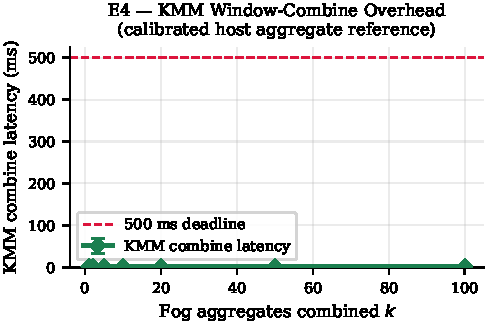
\includegraphics[width=1.0\linewidth]{../figures/exp4_kmm_combine.pdf}
    \caption{E4 KMM window-combine latency vs number of fog aggregates $k\in\{1,\ldots,100\}$. Latency scales linearly as $\approx1.474(k-1)$~ms, reaching $\approx$150~ms at $k=100$; all values remain within the 500~ms aggregation window.}
    \label{fig:e4-kmm}
    \end{figure}


    \subsection{Load Balancing Performance}
    \label{sec:eval-lb}

    \textbf{Setup.} Five fog nodes run 20 aggregation windows of 500~ms across five phases: normal operation (W1--5), $F_1$ burst (W6--10), $F_5$ failure (W11--13), recovery (W14--17), and $F_4$ burst (W18--20). Tasks split into latency-sensitive (LS, 100~ms deadline) and heavy-processing (HP, 500~ms deadline) classes. Six strategies are compared: S1 (random), S2 (round-robin), S3 (minimum workload), S4 (fixed CapScore weights), S5 (task-adaptive weights, no compatibility term), and S6 (proposed CapacityScore with compatibility term). Results are averaged over 20 seeds with 95\% CI. This experiment assumes instantaneous workload visibility to isolate strategy performance; gossip-induced staleness ($T_g = 500$~ms) is a separate concern evaluated in the fault-tolerance analysis (E6).

    \textbf{Results.} All six strategies complete 100\% of tasks; the discriminating metrics are deadline satisfaction and routing quality (Fig.~\ref{fig:e5-delegation-quality}). S6 achieves the highest deadline satisfaction at 78.77\% ($\pm$0.88\%), versus 78.35\% for S5, 77.28\% for S3, 77.01\% for S4, and 63.1--63.3\% for S1--S2. S6 also has the lowest mean waiting time at 101.11~ms ($\pm$3.94~ms), compared with 103--104~ms for S3--S5 and 790--854~ms for S1--S2. The 0.42 percentage-point margin between S6 and S5 lies within the confidence intervals; the advantage of the compatibility term is more conclusively demonstrated by the task-type results. S6 has the lowest bandwidth-utilization standard deviation ($\sigma_{BW}=0.225\pm0.005$ vs 0.239 for S5, 0.363 for S1--S2), accepting slightly less even scalar workload balance to reduce deadline misses.

    The task-type breakdown (Fig.~\ref{fig:e5-task-type}) explains the improvement. HP tasks miss deadlines at 15.18\% under S6, compared with 17.70--18.67\% for S3--S5 and 34--35\% for S1--S2. S6 assigns only 1.97\% of HP tasks to $F_3$ (the slowest node, which executes HP tasks in 600~ms, exceeding the deadline), versus 3.32--3.77\% for S3--S5 and 13.8--14.0\% for S1--S2. Phase-level results show S6 leads during normal operation (92.67\%), recovery (93.83\%), and $F_4$ burst (84.51\%). During $F_5$ failure, S5 performs best (48.22\%) while S6 drops to 37.93\%: the compatibility-heavy weighting ($w_4=0.45$) narrows candidate selection further when the pool shrinks due to failure. Deployments anticipating simultaneous failure and high arrival rates may reduce $w_4$ during degraded-mode operation.

    \textbf{Key takeaway.} CapacityScore improves deadline satisfaction by routing HP tasks away from structurally incompatible nodes and reducing bandwidth variance — not by completing more tasks, but by meeting deadlines under heterogeneous capacity and phased stress.

    \begin{figure}[htbp]
    \centering
    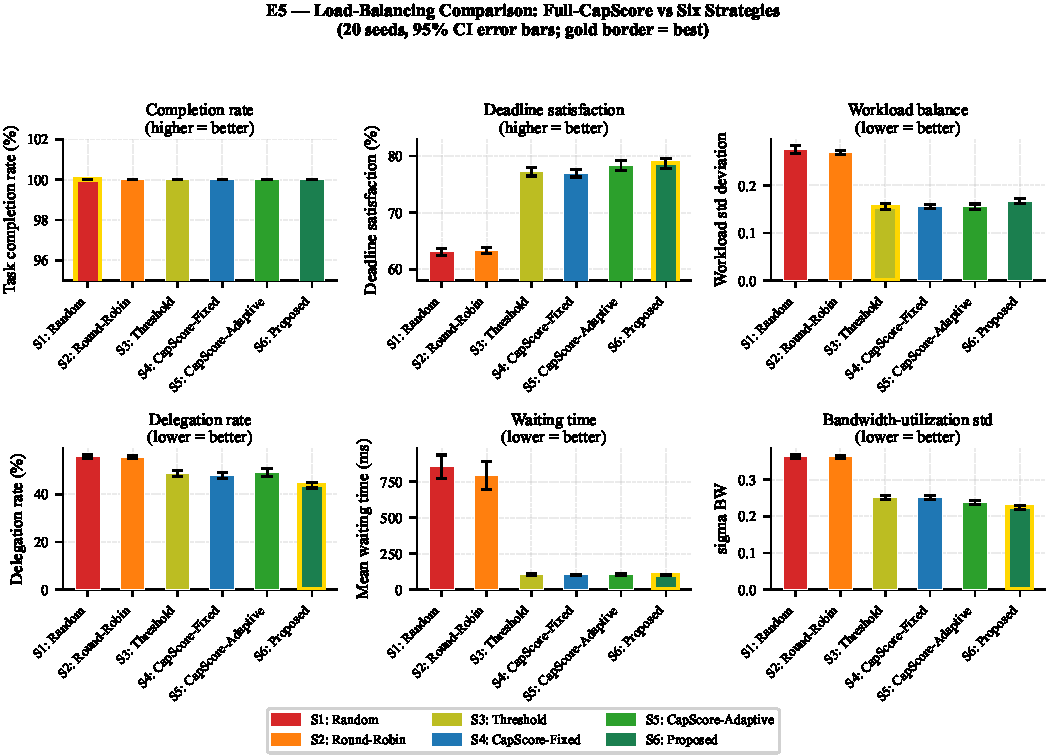
\includegraphics[width=1.0\linewidth]{../figures/e5_summary.pdf}
    \caption{Six-strategy load-balancing comparison: completion rate, deadline satisfaction, delegation rate, mean waiting time, and bandwidth-utilization standard deviation over 20 seeds with 95\% CI.}
    \label{fig:e5-delegation-quality}
    \end{figure}

    \begin{figure}[htbp]
    \centering
    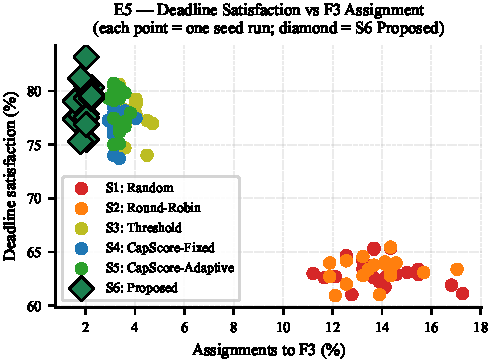
\includegraphics[width=1.0\linewidth]{../figures/e5_deadline_vs_f3.pdf}
    \caption{Deadline satisfaction vs HP task assignment rate to $F_3$ across S1--S6 over 20 seeds. S6 reduces HP tasks routed to the slowest node, improving overall deadline satisfaction.}
    \label{fig:e5-task-type}
    \end{figure}


    \subsection{Fault Tolerance and Security}
    \label{sec:eval-ft-sec}

    \textbf{Fault recovery (E6).} An analytical reading-loss model is evaluated over 30 seeds under three failure timings: failure at $t=0$~ms, 250~ms, and 450~ms within a 2000~ms observation window (400 total readings). Five baselines are compared (Table~\ref{tab:e6-baselines}): B1 gossip-only, B2 replication~\cite{liu2024replica}, B3 checkpoint sub-mechanism (derived from the RPC policy in~\cite{shahab2025sfc}), B4 multilayer detection~\cite{lee2022multilayer}, and B5 fog-clustering~\cite{mohammadi2023}. The proposed ACK+KMM method uses $T_{ack}=100\,\text{ms}$ plus $T_{KMM}=50\,\text{ms}$ provisioning, yielding 150~ms recovery latency.

    \begin{table}[htbp]
    \centering
    \caption{Fault-Tolerance Baselines}
    \label{tab:e6-baselines}
    \begin{tabular}{p{0.10\linewidth}p{0.82\linewidth}}
    \toprule
    & Simulator abstraction \\
    \midrule
    B1 & Gossip-only: failure detected after $rT_g=1500\,\text{ms}$; readings in outage window lost. \\
    B2 & Replication~\cite{liu2024replica}: each reading sent to primary and backup; zero loss, $2\times$ message cost. \\
    B3 & Checkpoint~\cite{shahab2025sfc} (checkpointing sub-mechanism of RPC isolated for comparison; 500~ms interval): readings after latest checkpoint lost until restore. \\
    B4 & Multilayer detection~\cite{lee2022multilayer}: sensor/fog/KMM detectors; earliest layer result used. \\
    B5 & Clustering~\cite{mohammadi2023}: coordinator detects failure and reroutes subsequent readings. \\
    \bottomrule
    \end{tabular}
    \end{table}

    In the worst case (failure at $t=0$), the proposed method loses $\approx$7.5\% of readings (30 of 400 during the 150~ms recovery window), versus 75\% for B1 gossip, $\approx$38\% for B5 clustering, and 25\% each for B3 and B4. B2 replication achieves zero loss at $2\times$ message overhead; the proposed method incurs only $1.055\times$. Fig.~\ref{fig:e6-fault} shows loss rates and recovery latency; Fig.~\ref{fig:e6-tradeoff} shows the loss--overhead tradeoff, where the proposed method is nearest to the origin among single-mechanism approaches.

    \begin{figure}[htbp]
    \centering
    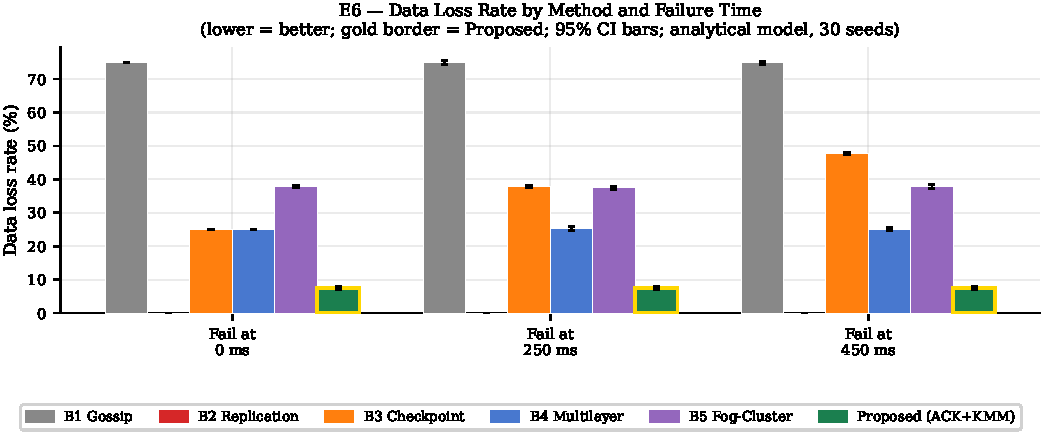
\includegraphics[width=1.0\linewidth]{../figures/exp6_data_loss.pdf}
    \caption{Data loss rate (upper) and recovery latency (lower) across six methods and three failure timings, averaged over 30 seeds with 95\% CI.}
    \label{fig:e6-fault}
    \end{figure}

    \begin{figure}[htbp]
    \centering
    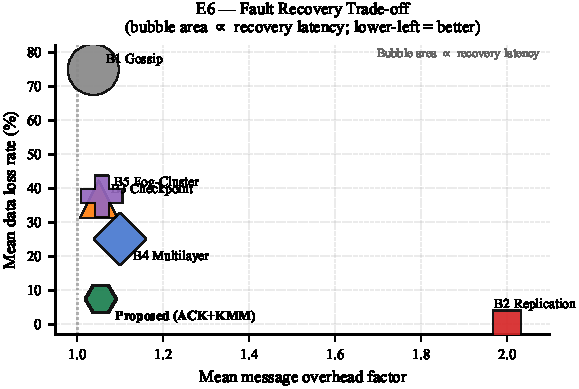
\includegraphics[width=1.0\linewidth]{../figures/exp6_tradeoff.pdf}
    \caption{Data loss vs message overhead tradeoff. The proposed ACK+KMM method (green) is closest to the origin among single-mechanism approaches.}
    \label{fig:e6-tradeoff}
    \end{figure}

    \textbf{Key exposure blast radius (E8).} Four compromise scenarios are evaluated analytically for 100 sensors across five fog nodes (20 per node). Under single-node enclave compromise ($F_1$), fog-scoped keys expose only 20 sensors versus all 100 under a global key (80\% reduction). Under backup-node compromise during active delegation ($F_4$ holding provisioned $k_{fogA}$), 40 sensors are exposed versus 100 (60\% reduction). KMM compromise exposes all 100 sensors under both designs since the KMM is the common trust anchor. Host OS memory access exposes zero sensors under both designs due to TEE enclave isolation. Fig.~\ref{fig:e8-blast} summarizes all scenarios.

    \textbf{Key takeaway.} Fog-scoped key isolation reduces the blast radius by 60--80\% in single-node compromise scenarios. The benefit does not extend to KMM compromise, the identified critical single point of failure.

    \begin{figure}[htbp]
    \centering
    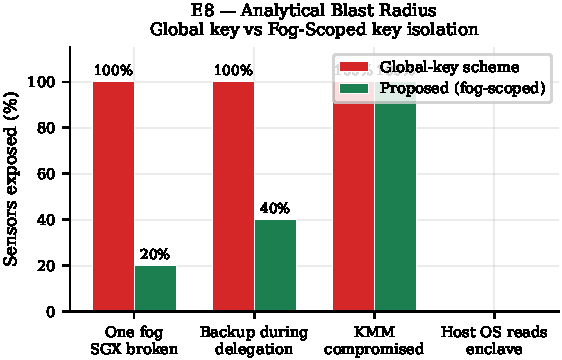
\includegraphics[width=1.0\linewidth]{../figures/exp8_blast_radius.pdf}
    \caption{Key exposure comparison between global and fog-scoped key designs across four threat scenarios (100 sensors, 20 per node).}
    \label{fig:e8-blast}
    \end{figure}

    \section{Future Work}

    A limitation of the present work is that the CapacityScore weights $(w_1, w_2, w_3, w_4)$ (Eq.~\eqref{eq:capacityscore}) and the compatibility term coefficients are fixed heuristics selected by task classification rather than learned from observed workload distributions. The strategy comparison in E5 demonstrates the advantage of the compatibility-aware term over simpler scoring strategies, but the specific weight values motivate data-driven adaptation. An important direction for future work is to replace the static weight table with an online learning mechanism---such as a contextual bandit or lightweight reinforcement learning policy---that adjusts weights based on observed deadline miss rates and node utilization histories across aggregation windows. Additionally, the workload update model in E5 uses a formula-based service time derived from static node profiles rather than a principled queuing model; extending the simulation to a discrete-event framework with explicit queue dynamics (e.g., M/M/$c$ per node) would produce more accurate estimates of redelegation rates and deadline miss probabilities at larger scales. The present evaluation covers five fog nodes, 20 windows, and 46--58 tasks per window depending on the stress phase; characterizing system behavior under hundreds of nodes and high-variance arrival rates represents a necessary step toward deployment-scale validation. Furthermore, the current Paillier-based aggregation layer supports only additive operations---sum, mean, and weighted sum. Future work will extend the scheme to CKKS-based slot batching to support multiplicative aggregation functions such as variance, product aggregation, and nonlinear statistics, and to provide approximate arithmetic over packed sensor vectors with formally bounded noise growth.

    The experimental evaluation rests on several simplifying assumptions that limit direct correspondence to real deployments. As described in Section~\ref{sec:eval-setup}, the TEE layer is emulated using OP-TEE on QEMU; no physical enclave boundary, sealing-key derivation, or remote attestation exchange is present in the prototype. The KMM provisioning latency $T_{KMM}=50\,\text{ms}$ is a fixed design parameter rather than a measured quantity. Future work should deploy the enclave layer on physical hardware---either an Intel SGX-capable processor using the Intel SGX SDK or Gramine, or an ARM TrustZone board running OP-TEE---and measure provisioning latency directly. Similarly, the end-to-end pipeline latency in E7 is derived entirely from hardcoded hardware-target constants; these estimates should be replaced by measurements on physical fog hardware equipped with AES-NI and a hardware TEE.

    The fault tolerance evaluation in E6 is based on an analytical reading-loss model that counts sensor readings falling within a fixed failure-to-recovery time window under three predetermined failure timings. This model does not capture cascading failures, partial node degradation, network partition effects, or the interaction between simultaneous sensor ACK timeouts and the gossip convergence process. Future work should validate the proposed ACK+KMM recovery mechanism under realistic fault injection using network emulation tools such as tc-netem or a containerized testbed, and should extend the failure model to cover correlated multi-node failures and transient network outages. The gossip protocol parameters---fan-out $k{=}3$, miss threshold $r{=}3$, and gossip interval $T_g{=}500\,\text{ms}$---are fixed throughout the evaluation; the probabilistic detection model derived from the Poisson failure process provides a design criterion ($T_g \leq \ln(20)/(\mu r)$ for $\beta=0.95$), but adaptive parameter selection under varying failure rates $\mu$ has not been investigated. The KMM is currently modeled as a single trusted authority; future work may investigate threshold or multi-party key management constructions that distribute the trust anchor across a quorum of KMM instances, reducing the exposure when the KMM is compromised. Finally, the present scheme provides computational confidentiality under the IND-CPA assumption for Paillier and AES-GCM but does not address what an honest-but-curious cloud observer can infer from the sequence of decrypted aggregates over time. Investigating differential privacy mechanisms for the aggregate output, or bounding the statistical leakage of the published aggregate stream, remains an open problem for future work.

    \section{Conclusion}

    This paper presented a fault-tolerant and load-balanced IIoT edge--fog architecture that jointly addresses three critical challenges: resource imbalance across heterogeneous fog nodes, fog-layer failures, and plaintext exposure during aggregation. The proposed framework integrates fog-scoped AES key isolation enforced by Trusted Execution Environments (TEEs), Paillier homomorphic slot aggregation with a zero-fill protocol for mid-window delegation, a three-layer fault-handling hierarchy combining per-reading TEE delegation, sensor ACK-timeout redirect, and gossip-based failure detection, and a task-aware CapacityScore selector that adapts routing decisions to the computational profile of each task type.

    Experimental evaluation across eight experiments demonstrated: constant per-window cloud storage independent of sensor count (E1); aggregate correctness under mid-window delegation in all 100 trials for both single-source and multi-source delegation (E3a--E3b); KMM combine latency scaling as $\approx1.474(k-1)$~ms, remaining within the 500~ms window for all tested $k\leq100$ (E4); the highest deadline satisfaction rate of 78.77\% and the lowest bandwidth-utilization variance among six compared strategies (E5); worst-case data loss reduced from 75\% under gossip-only detection to 7.5\% with the ACK+KMM mechanism at only $1.055\times$ message overhead (E6); and 60--80\% reduction in key-exposure blast radius relative to a global-key design under single-node compromise (E8).

    Future work will focus on validating the TEE enclave implementation on physical hardware (Intel SGX or ARM TrustZone), replacing the static CapacityScore weight table with an adaptive online learning policy, and extending the Paillier aggregation layer to CKKS-based slot batching for multiplicative and nonlinear aggregation functions.

    \bibliographystyle{IEEEtran}
    \bibliography{references}

    \end{document}
